% vim:spell spelllang=en:
\documentclass[a4paper,11pt]{article}
\usepackage[utf8]{inputenc}
%\usepackage{fullpage}
\usepackage{listings}
\usepackage{color}
\usepackage{url}
\usepackage{alltt}
\usepackage{multicol}
\usepackage{fancyhdr}
\usepackage{amsmath}
\usepackage{bussproofs}
\usepackage{comment}
\usepackage{inconsolata}
\usepackage{graphicx}

\usepackage{hyperref}
\definecolor{darkgreen}{rgb}{0.0,0.5,0.0}
\hypersetup{colorlinks=true,citecolor=darkgreen}

\renewcommand{\familydefault}{\sfdefault} % change to sans serif font

\newcommand{\seq}{\vdash}	% the sequent sign
\newcommand{\impl}{\supset} %logical connectives: implies, not, and, or
\renewcommand{\lnot}{\neg}
\renewcommand{\land}{\wedge}
\renewcommand{\lor}{\vee}
\newcommand{\sklabel}[2]{\langle#1\rangle^{#2}}

%Commands for constructing proof trees with bussproofs. See the chapter on the LK system for examples.
\newcommand{\UnaryInfCm}[1]{\UnaryInfC{$#1$}}
\newcommand{\BinaryInfCm}[1]{\BinaryInfC{$#1$}}
\newcommand{\RightLabelm}[1]{\RightLabel{$#1$}}
\newcommand{\AxiomCm}[1]{\AxiomC{$#1$}}

% Normal text in math mode ("math text")
\newcommand{\mt}[1]{\textnormal{#1}}
% CLI-style names,words,... within normal text
\newcommand{\cli}[1]{{\ttfamily {#1}}}

\usepackage[draft]{fixme}
\fxsetup{inline,nomargin,marginclue,theme=color,index}

\lstset{
  basicstyle=\small\ttfamily,
  breaklines=true,
%
  frame=leftline,
  framesep=1ex,
  framerule=1ex,
  rulecolor={\color[rgb]{0.8,0.8,0.8}},
%
  inputencoding=utf8,
  extendedchars=true,
  columns=flexible,
  morecomment=[l][\bfseries]{gapt> },
  literate=%
    {⊥}{{\ensuremath{\bot}}}1%
    {⊤}{{\ensuremath{\top}}}1%
    {∧}{{\ensuremath{\land}}}1%
    {⊃}{{\ensuremath{\impl}}}1%
    {∨}{{\ensuremath{\lor}}}1%
    {¬}{{\ensuremath{\neg}}}1%
    {∀}{{\ensuremath{\forall}}}1%
    {∃}{{\ensuremath{\exists}}}1%
    {ι}{{\ensuremath{\iota}}}1%
    {α}{{\ensuremath{\alpha}}}1%
    {β}{{\ensuremath{\beta}}}1%
    {τ}{{\ensuremath{\tau}}}1%
    {∈}{{\ensuremath{\in}}}1%
  }

% = clilisting environment
%
% This environment contains CLI interactions which are automatically evaluated
% using "sbt evalUserManual".
%
% Usage:
%
% \begin{clilisting}
% gapt> true
% res1: Boolean = true
% \end{clilisting}
%
% \begin{clilisting}[someCondition]
% gapt> this will only be executed if someCondition returns true
% \end{clilisting}
%
\lstnewenvironment{clilisting}[1][]{}{}

\setlength{\parindent}{0pt}
\setlength{\parskip}{4pt}
\setlength{\headheight}{14pt}
\setlength{\oddsidemargin}{1pt}
\setlength{\textwidth}{450pt}
%\setlength{\textheight}{600pt}

\pagestyle{fancy}
\lhead{GAPT -- User Manual}
\chead{}
\rhead{}

\begin{document}
\begin{titlepage}
\begin{center}

\hrule

\vspace*{20mm}

{\Huge GAPT}

\vspace*{5mm}

{\huge General Architecture for Proof Theory}

\vspace*{20mm}

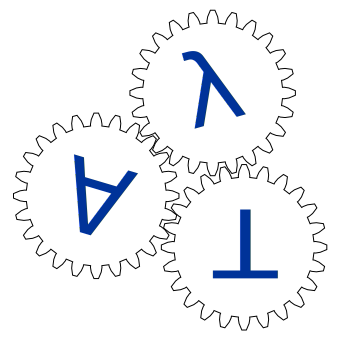
\includegraphics[keepaspectratio,width=5cm]{logo}

\vspace*{20mm}

{\Huge User manual}

\vspace*{10mm}
{\Large Version 2.0}
\vspace*{10mm}

{\Large \today}

\vspace*{20mm}

\hrule
\end{center}

\end{titlepage}

\listoffixmes

\tableofcontents
\vfill
\pagebreak

\section{Introduction}

GAPT is a generic architecture for proof transformations implemented in Scala.

The focus of GAPT are proof transformations (in contrast to proof assistants,
whose focus is proof formalization, and automated deduction systems, whose focus
is proof search). GAPT is used from a shell that provides access to the functionality
in the system in a way that is inspired by computer algebra systems: the basic
objects are formulas and (different kinds of) proofs which can be modified
by calling GAPT commands from the command line. In addition, there
is a graphical user interface that allows the user to view (and—to a certain extent—
modify) proofs in a flexible and visually appealing way.

The current functionality of GAPT includes data structures for formulas,
sequents, resolution proofs, sequent calculus proofs, expansion tree proofs and
algorithms for e.g.\ unification, proof Skolemization, cut-elimination, cut
elimination by resolution~\cite{Baaz00CutElimination},
cut-introduction~\cite{Hetzl2012}, etc.

\section{Download and execution}

There are three ways you can obtain GAPT:

\begin{enumerate}

\item {\bfseries The recommended way:}  You can download a package of the current
version of GAPT at~\url{https://logic.at/gapt/}.  After extracting
the \texttt{tar.gz}-file, you will find a shell script \texttt{gapt.sh}.

Running this script will start the command line interface of GAPT:
\begin{lstlisting}
./gapt.sh
\end{lstlisting}

\item If you are adventurous, you can also download an unstable development
  version from github:
\begin{lstlisting}
git clone https://github.com/gapt/gapt
cd gapt
sbt console
\end{lstlisting}

\item If you like GAPT and want to use it as a library in your Scala project,
  it is available as a Maven artifact on JCenter.  All you need to do is add
  one line to your \verb,build.sbt,:
\begin{lstlisting}
libraryDependencies += "at.logic.gapt" %% "gapt" % "2.0"
\end{lstlisting}

\end{enumerate}

The command line interface of GAPT is an interactive Scala shell.  This means
that all functionality of Scala is available to you.  In particular it is easy
to write Scala scripts that use the functionality of GAPT.

You don't need to know anything about Scala to try out the examples in this
manual, but if you do want to learn more about Scala we recommend the book
``Programming in Scala''~\cite{odersky2008programming}.

Interactions with the Scala shell are typeset in the following way:
\begin{clilisting}
gapt> println("Hello, world!")
Hello, world!

\end{clilisting}
Here, {\bfseries \cli{println("Hello, world!")}} is the user input, and \texttt{Hello,
world!} is the output from the Scala shell.

If you want to consult the in-depth API documentation of a function, you can
use the \cli{help} command:
\begin{clilisting}
gapt> help(containsQuantifierOnLogicalLevel)

\end{clilisting}

\subsection{System requirements}
\label{sec:sysreq}

To run GAPT you need to have Java 7 (or higher) installed.

GAPT contains interfaces to the following automated reasoning systems. Installing
them is optional. If GAPT does not find the executables in the path, the
functionality of these systems will not be available.

\begin{itemize}
\item Prover9 (\url{http://www.cs.unm.edu/~mccune/mace4/download/}) - make sure
  the commands \texttt{prover9} and \texttt{prooftrans} are available.
\item E theorem prover (\url{http://eprover.org/})
\item Vampire 4.0 (\url{http://www.vprover.org/})
\item LeanCoP (\url{http://leancop.de/})
\item VeriT (\url{http://www.verit-solver.org/})
\item Z3 (\url{https://github.com/Z3Prover/z3})
\item MiniSAT (\url{http://minisat.se/})
\item Glucose (\url{http://www.labri.fr/perso/lsimon/glucose/})
\item Sat4J (\url{http://sat4j.org/})
\item OpenWBO (\url{http://sat.inesc-id.pt/open-wbo/})
\item CVC4 (\url{http://cvc4.cs.nyu.edu/web/})
\end{itemize}

\section{Data structures}

\subsection{Formulas}

Formulas, terms, and other expressions are are represented as lambda terms in
simple type theory.  Terms and formulas of first-order logic and schematic
first-order logic are hence encoded as lambda terms, these form regular
subsets.

You can enter formulas by parsing them with the prover9~\cite{Prover9Input} parser:
%
\begin{clilisting}
gapt> val H = parseFormula( "(all x (P(x,f(x)) -> (exists y P(x,y))))" )
H: at.logic.gapt.expr.FOLFormula = ∀x.(P(x,f(x))⊃∃y.P(x,y))

\end{clilisting}
%
The prover9 syntax was also extended to higher-order logic, where type declarations are added:
%
\begin{clilisting}
gapt> val I = parseLLKFormula ( "var P:o>i>o; const f:o>i; var x:o; var y:i; (all x (P(x,f(x))) -> (exists y P(x,y)))" )
I: at.logic.gapt.expr.HOLFormula = ∀x:o.(P(x,f(x))⊃∃y.P(x,y))

\end{clilisting}

Please refer to Appendix~\ref{app:formulasyntax} for a full description of the languages the parsers accept.

A collection of formula sequences can be found in the file \cli{examples/FormulaSequences.scala}.
Have a look at this code to see how to compose formulas without the parser.
You can generate instances of these formula sequences by entering, e.g.,
%
\begin{clilisting}
gapt> val f = BussTautology( 5 )
f: at.logic.gapt.proofs.HOLSequent = ((((((c_1∨d_1)∧(c_2∨d_2))∧(c_3∨d_3))∧(c_4∨d_4))⊃c_5)∨(((((c_1∨d_1)∧(c_2∨d_2))∧(c_3∨d_3))∧(c_4∨d_4))⊃d_5)), (((((c_1∨d_1)∧(c_2∨d_2))∧(c_3∨d_3))⊃c_4)∨((((c_1∨d_1)∧(c_2∨d_2))∧(c_3∨d_3))⊃d_4)), ((((c_1∨d_1)∧(c_2∨d_2))⊃c_3)∨(((c_1∨d_1)∧(c_2∨d_2))⊃d_3)), (((c_1∨d_1)⊃c_2)∨((c_1∨d_1)⊃d_2)), (c_1∨d_1) :- c_5, d_5

\end{clilisting}

\subsection{Proofs}\label{sec:entering_proofs}

There are various possibilities for entering proofs into the system. The most
basic one is a direct top-down proof-construction using the constructors
of the inference rules.
\begin{clilisting}
gapt> val A = FOLAtom("A")
A: at.logic.gapt.expr.FOLAtom = A

gapt> val B = FOLAtom("B")
B: at.logic.gapt.expr.FOLAtom = B

gapt> val F1 = B --> (A & B)
F1: at.logic.gapt.expr.FOLFormula = (B⊃(A∧B))

gapt> val F2 = A & B
F2: at.logic.gapt.expr.FOLFormula = (A∧B)

\end{clilisting}
%
We start with the axioms:
%
\begin{clilisting}
gapt> val p1 = LogicalAxiom(A)
p1: at.logic.gapt.proofs.lk.LogicalAxiom =
[p1] A :- A    (LogicalAxiom(A))

gapt> val p2 = LogicalAxiom(B)
p2: at.logic.gapt.proofs.lk.LogicalAxiom =
[p1] B :- B    (LogicalAxiom(B))

\end{clilisting}
%
These are joined by an $\land:\mathrm{right}$-inference. See Appendix~\ref{app:sequent_calculus}
for the formal definition of the sequent calculus used in GAPT.
\begin{clilisting}
gapt> val p3 = AndRightRule( p1, A, p2, B )
p3: at.logic.gapt.proofs.lk.AndRightRule =
[p3] A, B :- (A∧B)    (AndRightRule(p1, Suc(0), p2, Suc(0)))
[p2] B :- B    (LogicalAxiom(B))
[p1] A :- A    (LogicalAxiom(A))

\end{clilisting}
%
To finish the proof it remains to apply two $\impl:\mathrm{right}$-inferences:
%
\begin{clilisting}
gapt> val p4 = ImpRightRule( p3, B, F2 )
p4: at.logic.gapt.proofs.lk.ImpRightRule =
[p4] A :- (B⊃(A∧B))    (ImpRightRule(p3, Ant(1), Suc(0)))
[p3] A, B :- (A∧B)    (AndRightRule(p1, Suc(0), p2, Suc(0)))
[p2] B :- B    (LogicalAxiom(B))
[p1] A :- A    (LogicalAxiom(A))

gapt> val p5 = ImpRightRule( p4, A, F1 )
p5: at.logic.gapt.proofs.lk.ImpRightRule =
[p5]  :- (A⊃(B⊃(A∧B)))    (ImpRightRule(p4, Ant(0), Suc(0)))
[p4] A :- (B⊃(A∧B))    (ImpRightRule(p3, Ant(1), Suc(0)))
[p3] A, B :- (A∧B)    (AndRightRule(p1, Suc(0), p2, Suc(0)))
[p2] B :- B    (LogicalAxiom(B))
[p1] A :- A    (LogicalAxiom(A))

\end{clilisting}
%
You can now view this proof by typing:
\begin{clilisting}
gapt> prooftool( p5 )

\end{clilisting}

The system comes with a collection of example proof sequences in the file
\cli{examples/ProofSequences.scala} which are generated in the above style.
Have a look at this code for more complicated proof constructions.
You can generate instances of these proof sequences by entering, e.g.,
%
\begin{clilisting}
gapt> val p = SumExampleProof( 5 )
p: at.logic.gapt.proofs.lk.LKProof =
[p27] ∀x.∀y.(P(s(x),y)⊃P(x,s(y))), P(s(s(s(s(s(0))))),0) :- P(0,s(s(s(s(s(0))))))    (ContractionLeftRule(p26, Ant(0), Ant(2)))
[p26] ∀x.∀y.(P(s(x),y)⊃P(x,s(y))), P(s(s(s(s(s(0))))),0), ∀x.∀y.(P(s(x),y)⊃P(x,s(y))) :- P(0,s(s(s(s(s(0))))))    (ForallLeftRule(p25, Ant(0), ∀y.(P(s(x),y)⊃P(x,s(y))), s(s(s(s(0)))), x))
[p25] ∀y.(P(s(s(s(s(s(0))))),y)⊃P(s(s(s(s(0)))),s(y))), P(s(s(s(s(s(0))))),0), ∀x.∀y.(P(s(x),y)⊃P(x,s(y))) :- P(0,s(s(s(s(s(0))))))    (ForallLeftRule(p24, Ant(0), (P(s(s(s(s(s(0))))),y)⊃P(s(s(s(s(0)))),s(y))), 0, y))
[p24] (P(s(s(s(s(s(0))))),0)⊃P(s(s(s(s(0)))),s(0))), P(s(s(s(s(s(0))))),0), ∀x.∀y.(P(s(x),y)⊃P(x,s(y))) :- P(0,s(s(s(s(s(0))))))    (ImpLeftRule(p1, Suc(0), p23, Ant(1)))
[p23] ∀x.∀y.(P(s(x),y)⊃P(x,s(y))), P(s(s(s(s(0)))),s(0)...
\end{clilisting}

\section{Feature walkthrough}

\subsection{SAT solver interface}
%
The following shows an example session, using the Sat4j SAT solver
to verify validity and satisfiability, and query the thus obtained models.
Consider the {\em pigeon hole principle for $(m, n)$, $\mathrm{PHP}_{m,n}$}, which states that if $m$ pigeons
are put into $n$ holes, then there is a hole which contains two pigeons. It is valid
iff $m>n$. $\neg\mathrm{PHP}_{m,n}$ states that when putting $m$ pigeons into $n$ holes, there
is no hole containing two pigeons. This is satisfiable iff $m\leq n$.
\begin{clilisting}
gapt> Sat4j isValid PigeonHolePrinciple(3, 2)
res3: Boolean = true

\end{clilisting}
shows\footnote{In Scala, \cli{Sat4j isValid formula} is syntactic sugar for \cli{Sat4j.isValid(formula)}.} that $\mathrm{PHP}_{3,2}$ is valid, and
\begin{clilisting}
gapt> Sat4j isValid PigeonHolePrinciple(3, 3)
res4: Boolean = false

\end{clilisting}
shows that $\mathrm{PHP}_{3,3}$ is not valid.
Furthermore,
\begin{clilisting}
gapt> val Some(m) = Sat4j solve -PigeonHolePrinciple(3, 3)
m: at.logic.gapt.models.Interpretation =
R(p_1,h_1) -> false
R(p_1,h_2) -> false
R(p_1,h_3) -> true
R(p_2,h_1) -> true
R(p_2,h_2) -> false
R(p_2,h_3) -> false
R(p_3,h_1) -> false
R(p_3,h_2) -> true
R(p_3,h_3) -> false

\end{clilisting}
yields a model of $\neg\mathrm{PHP}_{3,3}$ that can be queried:
\begin{clilisting}
gapt> val p1 = PigeonHolePrinciple.atom(1, 1)
p1: at.logic.gapt.expr.FOLAtom = R(p_1,h_1)

gapt> val p2 = PigeonHolePrinciple.atom(2, 1)
p2: at.logic.gapt.expr.FOLAtom = R(p_2,h_1)

gapt> m.interpret(p1) // Is pigeon 1 in hole 1?
res5: Boolean = false

gapt> m.interpret(p2) // Is pigeon 2 in hole 1?
res6: Boolean = true

\end{clilisting}
We can also interpret quantifier-free formulas:
\begin{clilisting}
gapt> m.interpret( And(p1, p2) )
res7: Boolean = false

\end{clilisting}

We can also convert $\neg\mathrm{PHP}_{3,3}$ into DIMACS format:
\begin{clilisting}
gapt> val (cnf, _, _) = structuralCNF(-PigeonHolePrinciple(3,3), generateJustifications=false, propositional=true)
cnf: Set[at.logic.gapt.proofs.HOLClause] = Set( :- R(p_3,h_1), R(p_3,h_2), R(p_3,h_3), R(p_3,h_2), R(p_2,h_2) :- , R(p_2,h_3), R(p_1,h_3) :- , R(p_3,h_3), R(p_2,h_3) :- ,  :- R(p_2,h_1), R(p_2,h_2), R(p_2,h_3), R(p_3,h_3), R(p_1,h_3) :- , R(p_2,h_1), R(p_1,h_1) :- , R(p_3,h_2), R(p_1,h_2) :- , R(p_3,h_1), R(p_1,h_1) :- , R(p_3,h_1), R(p_2,h_1) :- , R(p_2,h_2), R(p_1,h_2) :- ,  :- R(p_1,h_1), R(p_1,h_2), R(p_1,h_3))

gapt> val encoding = new DIMACSEncoding
encoding: at.logic.gapt.formats.dimacs.DIMACSEncoding = DIMACSEncoding()

gapt> writeDIMACS(encoding encodeCNF cnf)
res8: String =
"p cnf 9 12
1 2 3 0
-2 -4 0
-5 -6 0
-3 -5 0
7 4 5 0
-3 -6 0
-7 -8 0
-2 -9 0
-1 -8 0
-1 -7 0
-4 -9 0
8 9 6 0
"

\end{clilisting}

If you want to know which variable in the DIMACS output corresponds to which
atom in GAPT, you can query the \cli{DIMACSEncoding} object:
\begin{clilisting}
gapt> encoding decodeAtom 1
res9: at.logic.gapt.expr.HOLAtom = R(p_3,h_1)

\end{clilisting}

GAPT also supports other SAT solvers such as MiniSAT or Glucose out of the box:
\begin{clilisting}[MiniSAT.isInstalled]
gapt> MiniSAT isValid PigeonHolePrinciple(3,2)
res10: Boolean = true

\end{clilisting}
\begin{clilisting}[Glucose.isInstalled]
gapt> Glucose isValid PigeonHolePrinciple(3,2)
res11: Boolean = true

\end{clilisting}

If you have another DIMACS-compliant solver installed or want to pass extra
options to the SAT solver, you can pass a custom command to GAPT as well:
\begin{clilisting}[MiniSAT.isInstalled]
gapt> val solver = new ExternalSATSolver("minisat", "-mem-lim=1024")
solver: at.logic.gapt.provers.sat.ExternalSATSolver = ExternalSATSolver("minisat", "-mem-lim=1024")

gapt> solver isValid PigeonHolePrinciple(3,2)
res12: Boolean = true

\end{clilisting}

\subsection{MaxSAT solver interface}

The MaxSAT interface supports generating optimal solutions for weighted partial
MaxSAT instances: these consist of a list of hard clauses, which must be
satisfied in the solution; and a list of weighted soft clauses, where weight of
the satisfied soft clauses must be maximized.  See \cite{Argelich2008First}
for an overview.

Let us solve a simple example using the MaxSAT solver from SAT4J:

\begin{clilisting}
gapt> val Seq(a,b,c) = Seq("a","b","c") map {FOLAtom(_)}
a: at.logic.gapt.expr.FOLAtom = a
b: at.logic.gapt.expr.FOLAtom = b
c: at.logic.gapt.expr.FOLAtom = c

gapt> MaxSat4j.solve(hard = a|b|c, soft = Seq(-a -> 4, -b -> 3))
res13: Option[at.logic.gapt.models.Interpretation] =
Some(a -> false
b -> false
c -> true)

\end{clilisting}

GAPT also supports other MaxSAT solvers out of the box, just write
\cli{OpenWBO} or \cli{ToySolver} instead of \cli{MaxSat4j}.

\subsection{SMT solver interface}

The SMT solver interface in GAPT supports validity queries for \verb,QF_UF,
formulas.  For example we can check whether a quantifier-free formula is a
quasi-tautology using veriT:
\begin{clilisting}
gapt> val f = parseFormula("(a=b | a=c) & P(c) & P(b) -> P(a)")
f: at.logic.gapt.expr.FOLFormula = (((a=b∨a=c)∧(P(c)∧P(b)))⊃P(a))

\end{clilisting}

\begin{clilisting}[VeriT.isInstalled]
gapt> VeriT isValid f
res14: Boolean = true

\end{clilisting}

GAPT also supports Z3 and CVC4 out of the box (if they are installed):
\begin{clilisting}[Z3.isInstalled && CVC4.isInstalled]
gapt> Z3 isValid f
res15: Boolean = true

gapt> CVC4 isValid f
res16: Boolean = true

\end{clilisting}

You can export \verb,QF_UF, formulas (or sequents) as SMT-LIB benchmarks;
note that we apply a drastic renaming to the constant symbols in order to
support arbitrary (even Unicode) names in GAPT:
\begin{clilisting}
gapt> val (benchmark, typeRenaming, constantRenaming) =                                 SmtLibExporter(Sequent() :+ f)
benchmark: String =
"(set-logic QF_UF)
(declare-sort t1 0)
(declare-fun f1 (t1) Bool)
(declare-fun f2 () t1)
(declare-fun f3 () t1)
(declare-fun f4 () t1)
(assert (not (=> (and (or (= f4 f2) (= f4 f3)) (and (f1 f3) (f1 f2))) (f1 f4))))
(check-sat)
"
typeRenaming: Map[at.logic.gapt.expr.TBase,at.logic.gapt.expr.TBase] = Map(o -> Bool, i -> t1)
constantRenaming: Map[at.logic.gapt.expr.Const,at.logic.gapt.expr.Const] = Map(a -> f4, P -> f1, b -> f2, c -> f3)

\end{clilisting}

We can also extract instances for basic equality axioms (reflexivity, symmetry,
and congruences) from veriT's proof output:
\begin{clilisting}[VeriT.isInstalled]
gapt> val Some(expansionSequent) = VeriT getExpansionSequent (Sequent() :+ f)
expansionSequent: at.logic.gapt.proofs.expansionTrees.ExpansionSequent = WeakQuantifier(∀x.∀y.(x=y⊃y=x), ArrayBuffer((WeakQuantifier(∀y.(a=y⊃y=a), ArrayBuffer((Atom(a=b)⊃Atom(b=a),b), (Atom(a=c)⊃Atom(c=a),c))),a))), WeakQuantifier(∀x1.∀y1.((x1=y1∧P(x1))⊃P(y1)), ArrayBuffer((WeakQuantifier(∀y1.((c=y1∧P(c))⊃P(y1)), ArrayBuffer((Atom(c=a)∧Atom(P(c))⊃Atom(P(a)),a))),c), (WeakQuantifier(∀y1.((b=y1∧P(b))⊃P(y1)), ArrayBuffer((Atom(b=a)∧Atom(P(b))⊃Atom(P(a)),a))),b))) :- Atom(a=b)∨Atom(a=c)∧Atom(P(c))∧Atom(P(b))⊃Atom(P(a))

gapt> extractInstances(expansionSequent) foreach println
(a=b⊃b=a)
(a=c⊃c=a)
((c=a∧P(c))⊃P(a))
((b=a∧P(b))⊃P(a))
(((a=b∨a=c)∧(P(c)∧P(b)))⊃P(a))

\end{clilisting}

\subsection{First-order theorem prover interface}

GAPT includes interfaces to several first-order theorem provers, such as
Prover9, E prover, and LeanCoP.  For Prover9 and E prover we can read back
resolution proofs, and construct LK and expansion proofs from them.  The
LeanCoP interface only supports expansion sequent extraction.

Here is how you can get all of these kinds of proofs using Prover9:
\begin{clilisting}
gapt> val sequent = existsclosure("p(0)" +: "p(x) -> p(s(x))" +: Sequent()                                 :+ "p(s(s(0)))" map parseFormula)
sequent: at.logic.gapt.proofs.HOLSequent = p(0), ∀x.(p(x)⊃p(s(x))) :- p(s(s(0)))

\end{clilisting}

\begin{clilisting}[Prover9.isInstalled]
gapt> Prover9 isValid sequent
res18: Boolean = true

gapt> Prover9 getRobinsonProof sequent
res19: Option[at.logic.gapt.proofs.resolution.ResolutionProof] =
Some([p11]  :-     (Resolution(p6, Suc(0), p10, Ant(0)))
[p10] p(s(0)) :-     (Resolution(p7, Suc(0), p9, Ant(0)))
[p9] p(s(s(0))) :-     (Instance(p8, Substitution()))
[p8] p(s(s(0))) :-     (InputClause(p(s(s(0))) :- ))
[p7] p(s(0)) :- p(s(s(0)))    (Instance(p4, Substitution(v0 -> s(0))))
[p6]  :- p(s(0))    (Resolution(p2, Suc(0), p5, Ant(0)))
[p5] p(0) :- p(s(0))    (Instance(p4, Substitution(v0 -> 0)))
[p4] p(v0) :- p(s(v0))    (Instance(p3, Substitution(x -> v0)))
[p3] p(x) :- p(s(x))    (InputClause(p(x) :- p(s(x))))
[p2]  :- p(0)    (Instance(p1, Substitution()))
[p1]  :- p(0)    (InputClause( :- p(0)))
)

gapt> Prover9 getLKProof sequent
res20: Option[at.logic.gapt.proofs.lk.LKProof] =
Some([p19] ∀x.(p(x)⊃p(s(x))), p(0) :- p(s(s(0)))    (ContractionLeftRule(p18, Ant(2), Ant(1)))
[p18] p(0), ∀x.(p(x)⊃p(s(x))), ∀x.(p(x)⊃p(s(x))) :- p(s(s(0)))    (CutRule(p9, Suc(0), p17, Ant(1)))
[p17] ∀x.(p(x)⊃p(s(x))), p(s(0)) :- p(s(s(0)))    (CutRule(p14, Suc(0), p16, Ant(0)))
[p16] p(s(s(0))) :- p(s(s(0)))    (ContractionRightRule(p15, Suc(0), Suc(1)))
[p15] p(s(s(0))) :- p(s(s(0))), p(s(s(0)))    (WeakeningRightRule(p10, p(s(s(0)))))
[p14] ∀x.(p(x)⊃p(s(x))), p(s(0)) :- p(s(s(0)))    (ContractionLeftRule(p13, Ant(0), Ant(1)))
[p13] ∀x.(p(x)⊃p(s(x))), ∀x.(p(x)⊃p(s(x))), p(s(0)) :- p(s(s(0)))    (WeakeningLeftRule(p12, ∀x.(p(x)⊃p(s(x)))))
[p12] ∀x.(p(x)⊃p(s(x))), p(s(0)) :- p(s(s(0)))    (ForallLeftRule(p11, Ant(0), (p(x)⊃p(s(x))), s(0...
gapt> Prover9 getExpansionSequent sequent
res21: Option[at.logic.gapt.proofs.expansionTrees.ExpansionSequent] = Some(Atom(p(0)), WeakQuantifier(∀x.(p(x)⊃p(s(x))), List((Atom(p(0))⊃Atom(p(s(0))),0), (Atom(p(s(0)))⊃Atom(p(s(s(0)))),s(0)))) :- Atom(p(s(s(0)))))

\end{clilisting}

All of the above works with E prover (\cli{EProver}) and Vampire
(\cli{Vampire}) as well, we will just show \cli{EProver.getLKProof} as an
example:
\begin{clilisting}[EProver.isInstalled]
gapt> EProver getLKProof sequent
res22: Option[at.logic.gapt.proofs.lk.LKProof] =
Some([p19] p(0), ∀x.(p(x)⊃p(s(x))) :- p(s(s(0)))    (CutRule(p3, Suc(0), p18, Ant(1)))
[p18] ∀x.(p(x)⊃p(s(x))), p(0) :- p(s(s(0)))    (ContractionLeftRule(p17, Ant(2), Ant(0)))
[p17] ∀x.(p(x)⊃p(s(x))), p(0), ∀x.(p(x)⊃p(s(x))) :- p(s(s(0)))    (CutRule(p8, Suc(0), p16, Ant(1)))
[p16] ∀x.(p(x)⊃p(s(x))), p(s(0)) :- p(s(s(0)))    (CutRule(p13, Suc(0), p15, Ant(0)))
[p15] p(s(s(0))) :- p(s(s(0)))    (ContractionRightRule(p14, Suc(0), Suc(1)))
[p14] p(s(s(0))) :- p(s(s(0))), p(s(s(0)))    (WeakeningRightRule(p9, p(s(s(0)))))
[p13] ∀x.(p(x)⊃p(s(x))), p(s(0)) :- p(s(s(0)))    (ContractionLeftRule(p12, Ant(0), Ant(1)))
[p12] ∀x.(p(x)⊃p(s(x))), ∀x.(p(x)⊃p(s(x))), p(s(0)) :- p(s(s(0)))    (WeakeningLeftRule(p11, ∀x.(p(x)⊃p(s(x)))))
[p11] ∀x.(p(x)⊃p(...
\end{clilisting}

Note that \cli{getLKProof} only works for sequents without strong quantifiers
(i.e.\ sequents that are already Skolemized); however \cli{getExpansionSequent}
will happily return expansion sequents with Skolem quantifiers in that case:
\begin{clilisting}[Prover9.isInstalled]
gapt> val strong = ("(exists x all y P(x,y))" +: Sequent()                                     :+ "(all y exists x P(x,y))" map parseFormula)
strong: at.logic.gapt.proofs.Sequent[at.logic.gapt.expr.FOLFormula] = ∃x.∀y.P(x,y) :- ∀y.∃x.P(x,y)

gapt> Prover9 getExpansionSequent strong
res23: Option[at.logic.gapt.proofs.expansionTrees.ExpansionSequent] = Some(SkolemQuantifier(∃x.∀y.P(x,y), s_{0}, WeakQuantifier(∀y.P(s_{0},y), List((Atom(P(s_{0},s_{2})),s_{2})))) :- SkolemQuantifier(∀y.∃x.P(x,y), s_{2}, WeakQuantifier(∃x.P(x,s_{2}), List((Atom(P(s_{0},s_{2})),s_{0})))))

\end{clilisting}

The LeanCoP interface only supports the \cli{getExpansionSequent} method with
exactly one formula in the succedent:
\begin{clilisting}[LeanCoP.isInstalled]
gapt> LeanCoP getExpansionSequent sequent map {toDeep(_)}
res24: Option[at.logic.gapt.proofs.HOLSequent] = Some(p(0), ((p(0)⊃p(s(0)))∧(p(s(0))⊃p(s(s(0))))) :- p(s(s(0))))

\end{clilisting}

You can also export sequents in TPTP format if you want to pass them to other
provers manually:
\begin{clilisting}
gapt> TPTPFOLExporter.tptp_proof_problem_split(sequent)
res25: String =
"fof( formula0, axiom, 'p'('0') ).
fof( formula1, axiom, (! [X0] : ( 'p'(X0) => 'p'('s'(X0)) )) ).
fof( formula2, conjecture, 'p'('s'('s'('0'))) ).
"

\end{clilisting}

\subsection{Built-in tableaux prover}

GAPT contains a  built-in tableaux prover for propositional logic
which can be called with the command \texttt{solve.solvePropositional}, for example as in:
\begin{clilisting}
gapt> solve.solvePropositional(parseFormula("a -> (b -> a&b)"))
res26: Option[at.logic.gapt.proofs.lk.LKProof] =
Some([p5]  :- (a⊃(b⊃(a∧b)))    (ImpRightRule(p4, Ant(0), Suc(0)))
[p4] a :- (b⊃(a∧b))    (ImpRightRule(p3, Ant(1), Suc(0)))
[p3] a, b :- (a∧b)    (AndRightRule(p1, Suc(0), p2, Suc(0)))
[p2] b :- b    (LogicalAxiom(b))
[p1] a :- a    (LogicalAxiom(a))
)

\end{clilisting}


\subsection{Cut-elimination (Gentzen's method)}

The GAPT-system contains an implementation of reductive cut-elimination
\`{a} la Gentzen. It can be used as follows: first we load a proof $p$
with cuts (as in Appendix~\ref{sec.fileio}).
%
\begin{clilisting}
gapt> val p = XMLProofDatabaseParser( "examples/simple/fol1.xml.gz" ).proofs(0)._2
p: at.logic.gapt.proofs.lk.LKProof =
[p25] ∀x.∀y.(P(x,y)⊃Q(x,y)) :- ∃x.∃y.(¬Q(x,y)⊃¬P(x,y))    (CutRule(p13, Suc(0), p24, Ant(0)))
[p24] ∀x.∃y.(¬P(x,y)∨Q(x,y)) :- ∃x.∃y.(¬Q(x,y)⊃¬P(x,y))    (ForallLeftRule(p23, Ant(0), ∃y.(¬P(x,y)∨Q(x,y)), b, x))
[p23] ∃y.(¬P(b,y)∨Q(b,y)) :- ∃x.∃y.(¬Q(x,y)⊃¬P(x,y))    (ExistsLeftRule(p22, Ant(0), v, y))
[p22] (¬P(b,v)∨Q(b,v)) :- ∃x.∃y.(¬Q(x,y)⊃¬P(x,y))    (ExistsRightRule(p21, Suc(0), ∃y.(¬Q(x,y)⊃¬P(x,y)), b, x))
[p21] (¬P(b,v)∨Q(b,v)) :- ∃y.(¬Q(b,y)⊃¬P(b,y))    (ExistsRightRule(p20, Suc(0), (¬Q(b,y)⊃¬P(b,y)), v, y))
[p20] (¬P(b,v)∨Q(b,v)) :- (¬Q(b,v)⊃¬P(b,v))    (ImpRightRule(p19, Ant(1), Suc(0)))
[p19] (¬P(b,v)∨Q(b,v)), ¬Q(b,v) :- ¬P(b,v)    (OrLeftRule(p16, Ant(0), p18, Ant(1)))
[p18] ¬Q(b,v), Q(b,v) :-     (NegLeftRule(p17, Suc(0)))
[p17] Q(b,v) :- ...
\end{clilisting}
%
and then call the cut-elimination procedure:
\begin{clilisting}
gapt> val q = ReductiveCutElimination( p )
q: at.logic.gapt.proofs.lk.LKProof =
[p16] ∀x.∀y.(P(x,y)⊃Q(x,y)) :- ∃x.∃y.(¬Q(x,y)⊃¬P(x,y))    (ForallLeftRule(p15, Ant(0), ∀y.(P(x,y)⊃Q(x,y)), b, x))
[p15] ∀y.(P(b,y)⊃Q(b,y)) :- ∃x.∃y.(¬Q(x,y)⊃¬P(x,y))    (ForallLeftRule(p14, Ant(0), (P(b,y)⊃Q(b,y)), a, y))
[p14] (P(b,a)⊃Q(b,a)) :- ∃x.∃y.(¬Q(x,y)⊃¬P(x,y))    (ContractionRightRule(p13, Suc(0), Suc(1)))
[p13] (P(b,a)⊃Q(b,a)) :- ∃x.∃y.(¬Q(x,y)⊃¬P(x,y)), ∃x.∃y.(¬Q(x,y)⊃¬P(x,y))    (ImpLeftRule(p6, Suc(0), p12, Ant(0)))
[p12] Q(b,a) :- ∃x.∃y.(¬Q(x,y)⊃¬P(x,y))    (ExistsRightRule(p11, Suc(0), ∃y.(¬Q(x,y)⊃¬P(x,y)), b, x))
[p11] Q(b,a) :- ∃y.(¬Q(b,y)⊃¬P(b,y))    (ExistsRightRule(p10, Suc(0), (¬Q(b,y)⊃¬P(b,y)), a, y))
[p10] Q(b,a) :- (¬Q(b,a)⊃¬P(b,a))    (ImpRightRule(p9, Ant(0), Suc(0)))
[p9] ¬Q(b,a), Q(b,a) :- ¬P(b,a)    (WeakeningRightRule(p...
\end{clilisting}


\subsection{Skolemization}

Skolemization consists of replacing the variables bound by strong quantifiers in the end-sequent of a proof
by new function symbols thus obtaining a validity-equivalent sequent. In the GAPT-system Skolemization
is implemented for proofs and can be used, e.g.~as follows:
%
\begin{clilisting}
gapt> val Seq(x, y) = Seq("x", "y") map {FOLVar(_)}
x: at.logic.gapt.expr.FOLVar = x
y: at.logic.gapt.expr.FOLVar = y

gapt> val Pxy = FOLAtom("P", x, y)
Pxy: at.logic.gapt.expr.FOLAtom = P(x,y)

gapt> var p: LKProof = LogicalAxiom(Pxy)
p: at.logic.gapt.proofs.lk.LKProof =
[p1] P(x,y) :- P(x,y)    (LogicalAxiom(P(x,y)))

gapt> p = ExistsRightRule(p, Ex(x, Pxy), x)
p: at.logic.gapt.proofs.lk.LKProof = [p2] P(x,y) :- ∃x.P(x,y)    (ExistsRightRule(p1, Suc(0), P(x,y), x, x))
[p1] P(x,y) :- P(x,y)    (LogicalAxiom(P(x,y)))

gapt> p = ForallLeftRule(p, All(y, Pxy), y)
p: at.logic.gapt.proofs.lk.LKProof = [p3] ∀y.P(x,y) :- ∃x.P(x,y)    (ForallLeftRule(p2, Ant(0), P(x,y), y, y))
[p2] P(x,y) :- ∃x.P(x,y)    (ExistsRightRule(p1, Suc(0), P(x,y), x, x))
[p1] P(x,y) :- P(x,y)    (LogicalAxiom(P(x,y)))

gapt> p = ForallRightRule(p, All(y, Ex(x, Pxy)), y)
p: at.logic.gapt.proofs.lk.LKProof = [p4] ∀y.P(x,y) :- ∀y.∃x.P(x,y)    (ForallRightRule(p3, Suc(0), y, y))
[p3] ∀y.P(x,y) :- ∃x.P(x,y)    (ForallLeftRule(p2, Ant(0), P(x,y), y, y))
[p2] P(x,y) :- ∃x.P(x,y)    (ExistsRightRule(p1, Suc(0), P(x,y), x, x))
[p1] P(x,y) :- P(x,y)    (LogicalAxiom(P(x,y)))

gapt> p = ExistsLeftRule(p, Ex(x, All(y, Pxy)), x)
p: at.logic.gapt.proofs.lk.LKProof = [p5] ∃x.∀y.P(x,y) :- ∀y.∃x.P(x,y)    (ExistsLeftRule(p4, Ant(0), x, x))
[p4] ∀y.P(x,y) :- ∀y.∃x.P(x,y)    (ForallRightRule(p3, Suc(0), y, y))
[p3] ∀y.P(x,y) :- ∃x.P(x,y)    (ForallLeftRule(p2, Ant(0), P(x,y), y, y))
[p2] P(x,y) :- ∃x.P(x,y)    (ExistsRightRule(p1, Suc(0), P(x,y), x, x))
[p1] P(x,y) :- P(x,y)    (LogicalAxiom(P(x,y)))

gapt> val q = skolemize(p)
q: at.logic.gapt.proofs.lk.LKProof =
[p3] ∀y.P(s_{0},y) :- ∃x.P(x,s_{1})    (ForallLeftRule(p2, Ant(0), P(s_{0},y), s_{1}, y))
[p2] P(s_{0},s_{1}) :- ∃x.P(x,s_{1})    (ExistsRightRule(p1, Suc(0), P(x,s_{1}), s_{0}, x))
[p1] P(s_{0},s_{1}) :- P(s_{0},s_{1})    (LogicalAxiom(P(s_{0},s_{1})))

\end{clilisting}


\subsection{Interpolation}

The command \texttt{ExtractInterpolant} extracts an interpolant from a sequent calculus proof which may contain atomic cuts and/or equality rules. Currently, we allow only reflexivity axioms, and axioms of the form $A \seq A$; $\bot \seq$, or $\seq \top$. The implementation is based on Lemma 6.5 of~\cite{Takeuti87Proof}. The method expects
a proof p and an arbitrary partition of the end-sequent $\Gamma \seq \Delta$ of p into a
``negative part'' $\Gamma_1\seq\Delta_1$ and a ``positive part'' $\Gamma_2 \seq \Delta_2$.
It returns a formula $I$ s.t.\ $\Gamma_1\seq\Delta_1, I$ and $I,\Gamma_2\seq\Delta_2$
are provable and $I$ contains only such predicate symbols that appear in both, $\Gamma_1\seq\Delta_1$
and $\Gamma_2\seq\Delta_2$. For instance, suppose pr is the following proof:
\begin{center}
	\begin{prooftree}
		\AxiomCm{P(a) \seq P(a)}
		\RightLabelm{(\mt{w:l})}
		\UnaryInfCm{a=b, P(a) \seq P(a)}
		\RightLabelm{\mt{=:r}}
		\UnaryInfCm{a=b, P(a) \seq P(b)}
	\end{prooftree}
\end{center}
First, we construct the proof pr:
\begin{clilisting}
gapt> val ca = FOLConst( "a" )
ca: at.logic.gapt.expr.FOLConst = a

gapt> val cb = FOLConst( "b" )
cb: at.logic.gapt.expr.FOLConst = b

gapt> val pa = FOLAtom( "P", List( ca ) )
pa: at.logic.gapt.expr.FOLAtom = P(a)

gapt> val pb = FOLAtom( "P", List( cb ) )
pb: at.logic.gapt.expr.FOLAtom = P(b)

gapt> val aeqb = Eq( ca, cb )
aeqb: at.logic.gapt.expr.FOLAtom = a=b

gapt> val axpa = LogicalAxiom( pa )
axpa: at.logic.gapt.proofs.lk.LogicalAxiom =
[p1] P(a) :- P(a)    (LogicalAxiom(P(a)))

gapt> val axpb = LogicalAxiom( pb )
axpb: at.logic.gapt.proofs.lk.LogicalAxiom =
[p1] P(b) :- P(b)    (LogicalAxiom(P(b)))

gapt> val proof = WeakeningLeftRule( axpa, aeqb )
proof: at.logic.gapt.proofs.lk.WeakeningLeftRule =
[p2] a=b, P(a) :- P(a)    (WeakeningLeftRule(p1, a=b))
[p1] P(a) :- P(a)    (LogicalAxiom(P(a)))

gapt> val pr = EqualityRightRule( proof, aeqb, Suc( 0 ), pb )
pr: at.logic.gapt.proofs.lk.EqualityRightRule =
[p3] a=b, P(a) :- P(b)    (EqualityRightRule(p2, Ant(0), Suc(0), List([2])))
[p2] a=b, P(a) :- P(a)    (WeakeningLeftRule(p1, a=b))
[p1] P(a) :- P(a)    (LogicalAxiom(P(a)))

\end{clilisting}
In order to apply interpolation, we need to specify a partition of the end-sequent into $\Gamma_1 \seq \Delta_1$ and $\Gamma_2 \seq \Delta_2$, i.e. into the negative (npart) and positive (ppart) part, respectively. In this case, we set $\Delta_1 = \{ P(b) \}$, $\Gamma_2 = \{ a=b, P(a) \}$ and $\Gamma_1 = \Delta_2 = \emptyset$.

Then we can call \texttt{ExtractInterpolant( pr, npart, ppart )}, which returns the interpolant $I = (a=b \impl \lnot P(a))$ of pr:
\begin{clilisting}
gapt> val I = ExtractInterpolant( pr, Seq( Suc( 0 ) ), Seq( Ant( 0 ), Ant( 1 ) ) )
I: at.logic.gapt.expr.HOLFormula = (a=b⊃¬P(a))

\end{clilisting}

\subsection{Expansion trees}

Expansion trees are a compact representation of cut-free proofs. They have originally been
introduced in~\cite{Miller87Compact}. GAPT contains an implementation of
expansion trees for higher-order logic including functions for extracting expansion
trees from proofs, for merging expansion trees, for pruning and transforming them
in various ways and for viewing them in a comfortable way in the graphical user interface.

An expansion tree contains the instances of the quantifiers for a formula. In order
to represent an LK-proof we use {\em expansion sequents}, i.e.~sequents of expansion trees.
We can obtain an expansion sequent for example by:
\begin{clilisting}
gapt> val p = SquareEdgesExampleProof( 4 )
p: at.logic.gapt.proofs.lk.LKProof =
[p40] ∀x.∀y.(P(x,y)⊃P(s(x),y)), P(0,0), ∀x.∀y.(P(x,y)⊃P(x,s(y))) :- P(s(s(s(s(0)))),s(s(s(s(0)))))    (ContractionLeftRule(p39, Ant(0), Ant(2)))
[p39] ∀x.∀y.(P(x,y)⊃P(s(x),y)), P(0,0), ∀x.∀y.(P(x,y)⊃P(s(x),y)), ∀x.∀y.(P(x,y)⊃P(x,s(y))) :- P(s(s(s(s(0)))),s(s(s(s(0)))))    (ForallLeftRule(p38, Ant(0), ∀y.(P(x,y)⊃P(s(x),y)), 0, x))
[p38] ∀y.(P(0,y)⊃P(s(0),y)), P(0,0), ∀x.∀y.(P(x,y)⊃P(s(x),y)), ∀x.∀y.(P(x,y)⊃P(x,s(y))) :- P(s(s(s(s(0)))),s(s(s(s(0)))))    (ForallLeftRule(p37, Ant(0), (P(0,y)⊃P(s(0),y)), 0, y))
[p37] (P(0,0)⊃P(s(0),0)), P(0,0), ∀x.∀y.(P(x,y)⊃P(s(x),y)), ∀x.∀y.(P(x,y)⊃P(x,s(y))) :- P(s(s(s(s(0)))),s(s(s(s(0)))))    (ImpLeftRule(p1, Suc(0), p36, Ant(1)))
[p36] ∀x.∀y.(P(x,y)⊃P(s(x),y)), P(s(0),0), ∀x.∀y.(P(x,y)⊃P(x,s(y))) :- P(s(s(s(s(0))))...
gapt> val E = LKToExpansionProof( p )
E: at.logic.gapt.proofs.expansionTrees.ExpansionSequent = WeakQuantifier(∀x.∀y.(P(x,y)⊃P(s(x),y)), List((WeakQuantifier(∀y.(P(0,y)⊃P(s(0),y)), List((Atom(P(0,0))⊃Atom(P(s(0),0)),0))),0), (WeakQuantifier(∀y.(P(s(0),y)⊃P(s(s(0)),y)), List((Atom(P(s(0),0))⊃Atom(P(s(s(0)),0)),0))),s(0)), (WeakQuantifier(∀y.(P(s(s(0)),y)⊃P(s(s(s(0))),y)), List((Atom(P(s(s(0)),0))⊃Atom(P(s(s(s(0))),0)),0))),s(s(0))), (WeakQuantifier(∀y.(P(s(s(s(0))),y)⊃P(s(s(s(s(0)))),y)), List((Atom(P(s(s(s(0))),0))⊃Atom(P(s(s(s(s(0)))),0)),0))),s(s(s(0)))))), Atom(P(0,0)), WeakQuantifier(∀x.∀y.(P(x,y)⊃P(x,s(y))), List((WeakQuantifier(∀y.(P(s(s(s(s(0)))),y)⊃P(s(s(s(s(0)))),s(y))), List((Atom(P(s(s(s(s(0)))),0))⊃Atom(P(s(s(s(s(0)))),s(0))),0), (Atom(P(s(s(s(s(0)))),s(0)))⊃Atom(P(s(s(s(s(0)))),s(s(0)))),s(0)), (Atom(P(s(s(s(s(...
\end{clilisting}
This expansion sequent can then be viewed in the graphical user interface by simply calling:
\begin{clilisting}
gapt> prooftool( E )

\end{clilisting}

A window then opens that displays the end-sequent of \cli{p}, i.e.\ the shallow
sequent of \cli{E}.  You can then selectively expand quantifiers by clicking on
them, see~\cite{Hetzl13Understanding} for a detailed description.

\subsection{Cut-elimination by resolution (CERES)}\label{sec:ceres}

Cut-elimination by resolution (CERES) is a method which simplifies the cut
 formulas in a proof: a proof with arbitrary cut-formulas is transformed
 into a proof with atomic cuts. Since Expansion Proofs can be extracted
 directly from a proof with quantifier-free cut-formulas, we can skip
 the elimination of atomic cuts which has a worst time complexity
 exponential in the size of the proof.

For instance, the example proof \texttt{Pi2Pigeonhole} formalizes
 the fact that given an aviary with two holes and an infinite number
 of pigeons, one hole has to house at least two pigeons. The pigeons and
 the holes are represented by numerals in unary notation with zero $0$ and
 successor $s$. The function symbol $f$ maps pigeons to holes, which allows us
 to state the mapping of pigeons to holes as
 $\forall x (f(x) = 0 \lor f(x) = s(0))$. The actual statement to prove is then
 $\exists x \exists y (s(x) \leq y \land f(x) = f(y))$. In order to prove it
 we also need to axiomatize $\leq$ with
 $\forall x \forall y (s(x) \leq y \impl x \leq y)$ and transitivity
 $\forall x \forall y (x \leq M(x,y) \land M(x,y) \leq y \impl x \leq y)$ in its
 skolemized form.

We can extract the cut formulas using the \texttt{cutFormulas} command and find two
 cuts on quantified formulas: $\forall x \exists y (x \leq y \land f(y) = 0)$
 and $\forall x \exists y (x \leq y \land f(y) = s(0))$. This corresponds to a
 case distinction for each of the two holes which may contain the collision.
The actual simplification is performed using the \texttt{CERES} command. Please note
 that the input proof must be regular and have a skolemized end-sequent. The
 commands \texttt{regularize} and \texttt{skolemize} provide this functionality,
 if necessary.

\begin{clilisting}[Prover9.isInstalled]
gapt> prooftool(Pi2Pigeonhole())

gapt> cutFormulas(Pi2Pigeonhole()) filter {containsQuantifier(_)} foreach println
∀x.∃y.(<=(x,y)∧f(y)=s(0))
∀x.∃y.(<=(x,y)∧f(y)=0)

gapt> val acnf = CERES(Pi2Pigeonhole())
acnf: at.logic.gapt.proofs.lk.LKProof =
[p486] ∀x.(f(x)=0∨f(x)=s(0)), ∀x.∀y.(<=(x,M(x,y))∧<=(y,M(x,y))), ∀x.∀y.(<=(s(x),y)⊃<=(x,y)) :- ∃x.∃y.(<=(s(x),y)∧f(x)=f(y))    (ContractionRightRule(p485, Suc(1), Suc(0)))
[p485] ∀x.(f(x)=0∨f(x)=s(0)), ∀x.∀y.(<=(x,M(x,y))∧<=(y,M(x,y))), ∀x.∀y.(<=(s(x),y)⊃<=(x,y)) :- ∃x.∃y.(<=(s(x),y)∧f(x)=f(y)), ∃x.∃y.(<=(s(x),y)∧f(x)=f(y))    (ContractionLeftRule(p484, Ant(3), Ant(2)))
[p484] ∀x.∀y.(<=(x,M(x,y))∧<=(y,M(x,y))), ∀x.∀y.(<=(s(x),y)⊃<=(x,y)), ∀x.(f(x)=0∨f(x)=s(0)), ∀x.(f(x)=0∨f(x)=s(0)) :- ∃x.∃y.(<=(s(x),y)∧f(x)=f(y)), ∃x.∃y.(<=(s(x),y)∧f(x)=f(y))    (ContractionLeftRule(p483, Ant(4), Ant(2)))
[p483] ∀x.∀y.(<=(s(x),y)⊃<=(x,y)), ∀x.(f(x)=0∨f(x)=s(0)), ∀x.∀y.(<=(x,M(x,y))∧<=(y,M(x,y))), ∀x.(f(x)=0∨f(x)=s(0)), ∀x.∀y.(<=(x,M(x,y))∧<=(y,M(x,y))) :- ∃x.∃y.(...
gapt> prooftool(acnf)

gapt> val et = LKToExpansionProof(acnf)
et: at.logic.gapt.proofs.expansionTrees.ExpansionSequent = WeakQuantifier(∀x.(f(x)=0∨f(x)=s(0)), List((Atom(f(M(v100,s(M(v100,v101))))=0)∨Atom(f(M(v100,s(M(v100,v101))))=s(0)),M(v100,s(M(v100,v101)))), (Atom(f(M(v100,v101))=0)∨Atom(f(M(v100,v101))=s(0)),M(v100,v101)), (Atom(f(M(s(M(v100,s(M(v100,v101)))),s(M(v100,v101))))=0)∨Atom(f(M(s(M(v100,s(M(v100,v101)))),s(M(v100,v101))))=s(0)),M(s(M(v100,s(M(v100,v101)))),s(M(v100,v101)))), (Atom(f(M(v100,s(M(s(M(v100,v101)),v1))))=0)∨Atom(f(M(v100,s(M(s(M(v100,v101)),v1))))=s(0)),M(v100,s(M(s(M(v100,v101)),v1)))), (Atom(f(M(s(M(v100,v101)),v1))=0)∨Atom(f(M(s(M(v100,v101)),v1))=s(0)),M(s(M(v100,v101)),v1)), (Atom(f(M(s(M(v100,s(M(s(M(v100,v101)),v1)))),s(M(s(M(v100,v101)),v1))))=0)∨Atom(f(M(s(M(v100,s(M(s(M(v100,v101)),v1)))),s(M(s(M(v100,v101)),...
gapt> prooftool(et)

\end{clilisting}

\subsection{Cut-introduction}\label{sec.cut-introduction}

The cut-introduction algorithm as described in~\cite{Hetzl2012,Hetzl14Algorithmic,Hetzl14Introducing} is
implemented in GAPT for introducing $\Pi_1$-cuts into a sequent calculus
proof. We will use as input one of the proofs generated by
the system, namely, \texttt{LinearExampleProof(9)}. But the user can also
write his own proofs (see Section~\ref{sec:entering_proofs})
and input them to the cut-introduction algorithm.

Take an example proof:
\begin{clilisting}
gapt> val p = LinearExampleProof(4)
p: at.logic.gapt.proofs.lk.LKProof =
[p18] ∀x.(P(x)⊃P(s(x))), P(0) :- P(s(s(s(s(0)))))    (ContractionLeftRule(p17, Ant(0), Ant(2)))
[p17] ∀x.(P(x)⊃P(s(x))), P(0), ∀x.(P(x)⊃P(s(x))) :- P(s(s(s(s(0)))))    (ForallLeftRule(p16, Ant(0), (P(x)⊃P(s(x))), 0, x))
[p16] (P(0)⊃P(s(0))), P(0), ∀x.(P(x)⊃P(s(x))) :- P(s(s(s(s(0)))))    (ImpLeftRule(p1, Suc(0), p15, Ant(1)))
[p15] ∀x.(P(x)⊃P(s(x))), P(s(0)) :- P(s(s(s(s(0)))))    (ContractionLeftRule(p14, Ant(0), Ant(2)))
[p14] ∀x.(P(x)⊃P(s(x))), P(s(0)), ∀x.(P(x)⊃P(s(x))) :- P(s(s(s(s(0)))))    (ForallLeftRule(p13, Ant(0), (P(x)⊃P(s(x))), s(0), x))
[p13] (P(s(0))⊃P(s(s(0)))), P(s(0)), ∀x.(P(x)⊃P(s(x))) :- P(s(s(s(s(0)))))    (ImpLeftRule(p2, Suc(0), p12, Ant(1)))
[p12] ∀x.(P(x)⊃P(s(x))), P(s(s(0))) :- P(s(s(s(s(0)))))    (ContractionLeftRule(p11, A...
\end{clilisting}
Then compute a proof with a single cut that contains a single quantifier by:
\begin{clilisting}
gapt> val q = CutIntroduction.compressLKProof( p,                                   DeltaTableMethod( manyQuantifiers=false ), verbose=true )
Total inferences in the input proof: 16
Quantifier inferences in the input proof: 4
End sequent: ∀x.(P(x)⊃P(s(x))), P(0) :- P(s(s(s(s(0)))))
Size of term set: 6
Smallest grammar of size 6:
Axiom: (τ)
Non-terminal vectors:
  (τ)
  (α_0)
Productions:
  τ -> -{P(0)}_a1

  τ -> -{∀x.(P(x)⊃P(s(x)))}_a0(s(α_0))

  τ -> -{∀x.(P(x)⊃P(s(x)))}_a0(α_0)

  τ -> {P(s(s(s(s(0)))))}_s0

  α_0 -> 0

  α_0 -> s(s(0))


Size of the canonical solution: 8
Size of the minimized solution: 4
CNF of minimized cut-formula number 0:
  P(α_0) :- P(s(s(α_0)))
Number of cuts introduced: 1
Total inferences in the proof with cut(s): 19
Quantifier inferences in the proof with cut(s): 5
q: Option[at.logic.gapt.proofs.lk.LKProof] =
Some([p19] ∀x.(P(x)⊃P(s(x))), P(0) :- P(s(s(s(s(0)))))    (CutRule(p10, Suc(0), p18, Ant(0)))
[p18] ∀α_0.(P(α_0)⊃P(s(s(α_0)))), P(0) :- P(s(s(s(s(0)))))    (ContractionLeftRule(p17, Ant(1), Ant(0)))
[p17] ∀α_0.(P(α_0)⊃P(s(s(α_0)))), ∀α_0.(P(α_0)⊃P(s(s(α_0)))), P(0) :- P(s(s(s(s(0)))))    (ForallLeftRule(p16, Ant(2), (P(α_0)⊃P(s(s(α_0)))), s(s(0)), α_0))
[p16] ∀α_0.(P(α_0)⊃P(s(s(α_0)))), P(0), (P(s(s(0)))⊃P(s(s(s(s(0)))))) :- P(s(s(s(s(0)))))    (ForallLeftRule(p15, Ant(0), (P(α_0)⊃P(s(s(α_0)))), 0, α_0))
[p15] (P(0)⊃P(s(s(0)))), P(0), (P(s(s(0)))⊃P(s(s(s(s(0)))))) :- P(s(s(s(s(0)))))    (ImpLeftRule(p11, Suc(0), p14, Ant(1)))
[p14] (P(s(s(0)))⊃P(s(s(s(s(0)))))), P(s(s(0))) :- P(s(s(s(s(0)))))    (ImpLeftRule(p12, Suc(0), p13, Ant(0)))
[p13] P...
\end{clilisting}
You can also try \texttt{DeltaTableMethod(manyQuantifiers=true)}, this will proceed as above but will
compute a single cut with a block of quantifiers.  The method \texttt{MaxSATMethod(1,2)}
uses a reduction to a MaxSAT problem and an external MaxSAT-solver for finding a
minimal grammar corresponding to a proof with a cut with two cuts, one with $1$
quantifier, one with $2$ quantifiers.

\subsection{Tree grammars}

The cut-introduction method described in Section~\ref{sec.cut-introduction} is
based on the use of certain tree grammars for representing Herbrand-disjunctions.
These are totally rigid acyclic tree grammars (TRATGs) and vectorial TRATGs (VTRATGs).
As shown in~\cite{Hetzl14Algorithmic}, these grammars are intimately related to
the structure of proofs with cuts.  GAPT contains an implementation of
these tree grammars, and given a finite tree language (i.e., a set of terms), is
able to automatically find a (V)TRATG that covers this language:

\begin{clilisting}[OpenWBO.isInstalled]
gapt> val lang = 1 to 18 map { Numeral(_) }
lang: scala.collection.immutable.IndexedSeq[at.logic.gapt.expr.FOLTerm] = Vector(s(0), s(s(0)), s(s(s(0))), s(s(s(s(0)))), s(s(s(s(s(0))))), s(s(s(s(s(s(0)))))), s(s(s(s(s(s(s(0))))))), s(s(s(s(s(s(s(s(0)))))))), s(s(s(s(s(s(s(s(s(0))))))))), s(s(s(s(s(s(s(s(s(s(0)))))))))), s(s(s(s(s(s(s(s(s(s(s(0))))))))))), s(s(s(s(s(s(s(s(s(s(s(s(0)))))))))))), s(s(s(s(s(s(s(s(s(s(s(s(s(0))))))))))))), s(s(s(s(s(s(s(s(s(s(s(s(s(s(0)))))))))))))), s(s(s(s(s(s(s(s(s(s(s(s(s(s(s(0))))))))))))))), s(s(s(s(s(s(s(s(s(s(s(s(s(s(s(s(0)))))))))))))))), s(s(s(s(s(s(s(s(s(s(s(s(s(s(s(s(s(0))))))))))))))))), s(s(s(s(s(s(s(s(s(s(s(s(s(s(s(s(s(s(0)))))))))))))))))))

gapt> val grammar = findMinimalGrammar(lang, 2)
grammar: at.logic.gapt.grammars.TratGrammar =
Axiom: τ
Non-terminals: τ, α_1, α_2
Productions:
  τ -> s(s(s(s(α_1))))
  τ -> s(α_1)
  α_1 -> s(s(α_2))
  α_1 -> s(α_2)
  α_1 -> α_2
  α_2 -> 0
  α_2 -> s(s(s(s(s(s(0))))))
  α_2 -> s(s(s(s(s(s(s(s(s(s(s(s(0))))))))))))

gapt> lang.toSet subsetOf grammar.language
res32: Boolean = true

\end{clilisting}

You can also find minimal sub-grammars that still generate certain terms:
\begin{clilisting}[OpenWBO.isInstalled]
gapt> minimizeGrammar(grammar, Set(1,2,4,5) map {Numeral(_)})
res33: at.logic.gapt.grammars.TratGrammar =
Axiom: τ
Non-terminals: τ, α_1, α_2
Productions:
  τ -> s(s(s(s(α_1))))
  τ -> s(α_1)
  α_1 -> s(α_2)
  α_1 -> α_2
  α_2 -> 0

\end{clilisting}

\vfill
\pagebreak
\begin{appendix}

\section{Proof systems}

\subsection{LK}\label{app:sequent_calculus}

The rules of LK are listed below. Proof trees are constructed top-down, starting with axioms and with each rule introducing new inferences. With the exception of the definition rules, the constructors of the rules only allow inferences that are actually valid. Note that the rules are presented here as if they always act upon the outermost formulas in the upper sequent, but this is only for convenience of presentation. The basic constructors actually require the user to specify on which concrete formulas the inference should be performed.

Apart from those basic constructors, there is also a multitude of convenience constructors that facilitate easier proof construction. Moreover, there are so-called macro rules that reduce several inferences to a single command (e.g. introducing quantifier blocks). See the API documentation of the individual rules for details.

\subsubsection*{Axioms}

\begin{multicols}{2}
\begin{prooftree}
\AxiomCm{}
\RightLabelm{(\mt{Logical axiom})}
\UnaryInfCm{A \seq A}
\end{prooftree}

\begin{prooftree}
\AxiomCm{}
\RightLabelm{\mt{$\top$ axiom}}
\UnaryInfCm{\seq \top}
\end{prooftree}

\begin{prooftree}
\AxiomCm{}
\RightLabelm{(\mt{Reflexivity axiom})}
\UnaryInfCm{\seq t = t}
\end{prooftree}

\begin{prooftree}
\AxiomCm{}
\RightLabelm{\mt{$\bot$ axiom}}
\UnaryInfCm{\bot \seq}
\end{prooftree}
\end{multicols}

\begin{prooftree}
\AxiomCm{}
\RightLabelm{\mt{Theory axiom}}
\UnaryInfCm{\Gamma \seq \Delta}
\end{prooftree}

Theory axioms may only contain atomic formulas.

\subsubsection*{Cut}

  \begin{prooftree}
  \AxiomCm{\Gamma \seq \Delta, A}
  \AxiomCm{A, \Sigma \seq \Pi}
  \RightLabelm{(\mt{cut})}
  \BinaryInfCm{\Gamma, \Sigma \seq \Delta, \Pi}
  \end{prooftree}

\subsubsection*{Structural rules}

\begin{multicols}{2}

  \subsubsection*{Left rules}

  \begin{prooftree}
  \AxiomCm{\Gamma \seq \Delta}
  \RightLabelm{(\mt{w:l})}
  \UnaryInfCm{A, \Gamma \seq \Delta}
  \end{prooftree}

  \begin{prooftree}
  \AxiomCm{A,A,\Gamma \seq \Delta}
  \RightLabelm{(\mt{c:l})}
  \UnaryInfCm{A,\Gamma\seq \Delta}
  \end{prooftree}

  \subsubsection*{Right rules}

  \begin{prooftree}
  \AxiomCm{\Gamma \seq \Delta}
  \RightLabelm{(\mt{w:r})}
  \UnaryInfCm{\Gamma \seq \Delta, A}
  \end{prooftree}

  \begin{prooftree}
  \AxiomCm{\Gamma \seq \Delta, A, A}
  \RightLabelm{(\mt{c:r})}
  \UnaryInfCm{\Gamma \seq \Delta, A}
  \end{prooftree}

\end{multicols}

\newpage

\subsubsection*{Propositional rules}

\begin{multicols}{2}

  \subsubsection*{Left rules}

  \begin{prooftree}
  \AxiomCm{A,B,\Gamma \seq \Delta}
  \RightLabelm{(\land\mt{:l})}
  \UnaryInfCm{A \land B,\Gamma \seq \Delta}
  \end{prooftree}

  \begin{prooftree}
  \AxiomCm{A, \Gamma \seq \Delta}
  \AxiomCm{B, \Sigma \seq \Pi}
  \RightLabelm{(\lor\mt{:l})}
  \BinaryInfCm{A \lor B, \Gamma, \Sigma \seq \Delta, \Pi}
  \end{prooftree}

  \begin{prooftree}
  \AxiomCm{\Gamma \seq \Delta, A}
  \RightLabelm{(\lnot\mt{:l})}
  \UnaryInfCm{\neg A, \Gamma \seq \Delta}
  \end{prooftree}

  \begin{prooftree}
  \AxiomCm{\Gamma \seq \Delta, A}
  \AxiomCm{B, \Sigma \seq \Pi}
  \RightLabelm{(\impl\mt{:l})}
  \BinaryInfCm{A \impl B, \Gamma, \Sigma \seq \Delta, \Pi}
  \end{prooftree}

  \subsubsection*{Right rules}

  \begin{prooftree}
  \AxiomCm{\Gamma \seq \Delta, A}
  \AxiomCm{\Sigma \seq \Pi, B}
  \RightLabelm{(\land\mt{:r})}
  \BinaryInfCm{\Gamma, \Sigma \seq \Delta, \Pi, A \land B}
  \end{prooftree}

  \begin{prooftree}
  \AxiomCm{\Gamma \seq \Delta, A, B}
  \RightLabelm{(\lor\mt{:r})}
  \UnaryInfCm{\Gamma \seq \Delta, A \lor B}
  \end{prooftree}

  \begin{prooftree}
  \AxiomCm{A, \Gamma\seq \Delta}
  \RightLabelm{(\lnot\mt{:r})}
  \UnaryInfCm{\Gamma \seq \Delta, \neg A}
  \end{prooftree}

  \begin{prooftree}
  \AxiomCm{A, \Gamma \seq \Delta, B}
  \RightLabelm{(\impl\mt{:r})}
  \UnaryInfCm{\Gamma \seq \Delta, A \impl B}
  \end{prooftree}

\end{multicols}

\subsubsection*{Quantifier rules}

\begin{multicols}{2}

  \subsubsection*{Left rules}

  \begin{prooftree}
  \AxiomCm{A[t/x], \Gamma \seq \Delta}
  \RightLabelm{(\forall\mt{:l})}
  \UnaryInfCm{\forall x A, \Gamma \seq \Delta}
  \end{prooftree}

  \begin{prooftree}
  \AxiomCm{A[y/x], \Gamma \seq \Delta}
  \RightLabelm{(\exists\mt{:l})}
  \UnaryInfCm{\exists x A, \Gamma \seq \Delta}
  \end{prooftree}

  \subsubsection*{Right rules}

  \begin{prooftree}
  \AxiomCm{\Gamma \seq \Delta, A[y/x]}
  \RightLabelm{(\forall\mt{:r})}
  \UnaryInfCm{\Gamma \seq \Delta, \forall x A}
  \end{prooftree}

  \begin{prooftree}
  \AxiomCm{\Gamma \seq \Delta, A[t/x]}
  \RightLabelm{(\exists\mt{:r})}
  \UnaryInfCm{\Gamma \seq \Delta, \exists x A}
  \end{prooftree}

\end{multicols}

The variable $y$ must not occur free in $\Gamma$, $\Delta$ or $A$. The term $t$ must avoid variable capture, i.e.\ it must not contain free occurrences of variables bound in $A$.

\subsubsection*{Equality rules}

\begin{multicols}{2}

  \subsubsection*{Left rules}

  \begin{prooftree}
  \AxiomCm{s = t, A[T/s], \Sigma \seq \Pi}
  \RightLabelm{(\mt{=:l})}
  \UnaryInfCm{s = t, A[T/t], \Sigma \seq \Pi}
  \end{prooftree}

  \begin{prooftree}
  \AxiomCm{s = t, A[T/t], \Sigma \seq \Pi}
  \RightLabelm{(\mt{=:l})}
  \UnaryInfCm{s = t, A[T/s], \Sigma \seq \Pi}
  \end{prooftree}

  \subsubsection*{Right rules}

  \begin{prooftree}
  \AxiomCm{s = t, \Sigma \seq \Pi, A[T/s]}
  \RightLabelm{(\mt{=:r})}
  \UnaryInfCm{s = t, \Sigma \seq \Pi, A[T/t]}
  \end{prooftree}

  \begin{prooftree}
  \AxiomCm{s = t, \Sigma \seq \Pi, A[T/t]}
  \RightLabelm{(\mt{=:r})}
  \UnaryInfCm{s = t, \Sigma \seq \Pi, A[T/s]}
  \end{prooftree}

\end{multicols}
Each equation rule replaces an arbitrary number of occurrences of $T$.

\subsubsection*{Definition rules}
\begin{center}
 \AxiomCm{A, \Gamma \seq \Delta}
 \RightLabelm{(\mt{def:l})}
 \UnaryInfCm{B, \Gamma \seq \Delta}
 \DisplayProof
 \AxiomCm{\Gamma \seq \Delta, A}
 \RightLabelm{(\mt{def:r})}
 \UnaryInfCm{\Gamma \seq \Delta, B}
 \DisplayProof
\end{center}
These definition rules are extremely liberal, as they allow the replacement of any formula by any other formula.

\subsubsection*{Induction}
The induction rule applies to arbitrary algebraic data types. Let $c_1,\dots,c_n$ be the constructors of a type and let $k_i$ be the arity of $c_i$. Let $F[x]$ be a formula with $x$ a free variable of the appropriate type. Then we call the sequent $\mathcal{S}_i := F[x_1],\dots,F[x_{k_i}], \Gamma_i \seq \Delta_i, F[c_i(x_1,\dots,x_{k_i})]$ the $i$-th induction step. In this case, the induction rule has the form
  \begin{prooftree}
    \AxiomCm{(\pi_1)}
    \noLine
    \UnaryInfCm{\mathcal{S}_1}
    \AxiomCm{(\pi_2)}
    \noLine
    \UnaryInfCm{\mathcal{S}_2}
    \AxiomCm{\dots}
    \AxiomCm{(\pi_n)}
    \noLine
    \UnaryInfCm{\mathcal{S}_n}
    \RightLabelm{(\mt{ind})}
    \QuaternaryInfC{$\Gamma \seq \Delta, \forall x F[x]$}
  \end{prooftree}

  In the case of the natural numbers, there are two constructors: $0$ of arity 0 and $s$ of arity 1. Consequently, the induction rule reduces to

  \begin{prooftree}
    \AxiomCm{(\pi_1)}
    \noLine
    \UnaryInfCm{\Gamma_1 \seq \Delta_1, F[0]}
    \AxiomCm{(\pi_2)}
    \noLine
    \UnaryInfCm{F[x], \Gamma_2 \seq \Delta_2, F[sx]}
    \RightLabelm{(\mt{ind})}
    \BinaryInfCm{\Gamma_1, \Gamma_2 \seq \Delta_1, \Delta_2, \forall x F[x]}
  \end{prooftree}

\subsection{Resolution}

\subsection*{Initial clauses}

\begin{prooftree}
\AxiomC{}\RightLabel{InputClause}
\UnaryInfC{$C$}
\end{prooftree}

\begin{prooftree}
\AxiomC{}\RightLabel{ReflexivityClause}
\UnaryInfC{$t=t$}
\end{prooftree}

\begin{prooftree}
\AxiomC{}\RightLabel{TautologyClause}
\UnaryInfC{$a \lor \neg a$}
\end{prooftree}

\subsection*{Structural rules}

\begin{prooftree}
\AxiomC{$a \lor a \lor C$}\RightLabel{Factor}
\UnaryInfC{$a \lor C$}
\end{prooftree}

\begin{prooftree}
\AxiomC{$C$}\RightLabel{Instance}
\UnaryInfC{$C \sigma$}
\end{prooftree}

\subsection*{Logical rules}

\begin{prooftree}
\AxiomC{$C \lor a$}
\AxiomC{$\neg a \lor D$}
\RightLabel{Resolution}
\BinaryInfC{$C \lor D$}
\end{prooftree}

\begin{prooftree}
\AxiomC{$C \lor t=s$}
\AxiomC{$l[t] \lor D$}
\RightLabel{Paramodulation}
\BinaryInfC{$C \lor l[s] \lor D$}
\end{prooftree}

\begin{prooftree}
\AxiomC{$C \lor t=s$}
\AxiomC{$l[s] \lor D$}
\RightLabel{Paramodulation}
\BinaryInfC{$C \lor l[t] \lor D$}
\end{prooftree}

\subsection{LKsk}

LKsk is a sequent calculus used in the CERES method for higher-order logic, see
\cite{Weller2010CERES} for an overview of both the calculus and the method.

LKsk operates on labelled formulas. A label $\ell$ is a finite list of terms, a labelled formula is a pair $(F, \ell)$, written as $\sklabel{F}{\ell}$. If $\ell$ is a label and $t$ a term, we write $\ell;t$ for the concatenation of $\ell$ and $t$.

\subsubsection*{Axioms}

\begin{multicols}{2}
\begin{prooftree}
\AxiomCm{}
\RightLabelm{(\mt{Logical axiom})}
\UnaryInfCm{\sklabel{A}{\ell_1} \seq \sklabel{A}{\ell_2}}
\end{prooftree}

\begin{prooftree}
\AxiomCm{}
\RightLabelm{\mt{$\top$ axiom}}
\UnaryInfCm{\seq \sklabel{\top}{\ell}}
\end{prooftree}

\begin{prooftree}
\AxiomCm{}
\RightLabelm{(\mt{Reflexivity axiom})}
\UnaryInfCm{\seq \sklabel{t = t}{\ell}}
\end{prooftree}

\begin{prooftree}
\AxiomCm{}
\RightLabelm{\mt{$\bot$ axiom}}
\UnaryInfCm{\sklabel{\bot}{\ell}\seq}
\end{prooftree}
\end{multicols}

\begin{prooftree}
\AxiomCm{}
\RightLabelm{\mt{Theory axiom}}
\UnaryInfCm{\sklabel{A_1}{\ell_1},\dots,\sklabel{A_m}{\ell_m} \seq \sklabel{B_1}{\ell'_1},\dots,\sklabel{B_n}{\ell'_n}}
\end{prooftree}

\subsubsection*{Cut}

  \begin{prooftree}
  \AxiomCm{\Gamma \seq \Delta, \sklabel{A}{\ell_1}}
  \AxiomCm{\sklabel{A}{\ell_2}, \Sigma \seq \Pi}
  \RightLabelm{(\mt{cut})}
  \BinaryInfCm{\Gamma, \Sigma \seq \Delta, \Pi}
  \end{prooftree}

  Note that the labels of the cut formulas do not need to be equal.

\subsubsection*{Structural rules}

\begin{multicols}{2}

  \subsubsection*{Left rules}

  \begin{prooftree}
  \AxiomCm{\Gamma \seq \Delta}
  \RightLabelm{(\mt{w:l})}
  \UnaryInfCm{\sklabel{A}{\ell}, \Gamma \seq \Delta}
  \end{prooftree}

  \begin{prooftree}
  \AxiomCm{\sklabel{A}{\ell},\sklabel{A}{\ell},\Gamma \seq \Delta}
  \RightLabelm{(\mt{c:l})}
  \UnaryInfCm{\sklabel{A}{\ell},\Gamma\seq \Delta}
  \end{prooftree}

  \subsubsection*{Right rules}

  \begin{prooftree}
  \AxiomCm{\Gamma \seq \Delta}
  \RightLabelm{(\mt{w:r})}
  \UnaryInfCm{\Gamma \seq \Delta, \sklabel{A}{\ell}}
  \end{prooftree}

  \begin{prooftree}
  \AxiomCm{\Gamma \seq \Delta, \sklabel{A}{\ell}, \sklabel{A}{\ell}}
  \RightLabelm{(\mt{c:r})}
  \UnaryInfCm{\Gamma \seq \Delta, \sklabel{A}{\ell}}
  \end{prooftree}

\end{multicols}

\subsubsection*{Propositional rules}

\begin{multicols}{2}

  \subsubsection*{Left rules}

  \begin{prooftree}
  \AxiomCm{\sklabel{A}{\ell},\sklabel{B}{\ell},\Gamma \seq \Delta}
  \RightLabelm{(\land\mt{:l})}
  \UnaryInfCm{\sklabel{A \land B}{\ell},\Gamma \seq \Delta}
  \end{prooftree}

  \begin{prooftree}
  \AxiomCm{\sklabel{A}{\ell}, \Gamma \seq \Delta}
  \AxiomCm{\sklabel{B}{\ell}, \Sigma \seq \Pi}
  \RightLabelm{(\lor\mt{:l})}
  \BinaryInfCm{\sklabel{A \lor B}{\ell}, \Gamma, \Sigma \seq \Delta, \Pi}
  \end{prooftree}

  \begin{prooftree}
  \AxiomCm{\Gamma \seq \Delta, \sklabel{A}{\ell}}
  \RightLabelm{(\lnot\mt{:l})}
  \UnaryInfCm{\sklabel{\neg A}{\ell}, \Gamma \seq \Delta}
  \end{prooftree}

  \begin{prooftree}
  \AxiomCm{\Gamma \seq \Delta, \sklabel{A}{\ell}}
  \AxiomCm{\sklabel{B}{\ell}, \Sigma \seq \Pi}
  \RightLabelm{(\impl\mt{:l})}
  \BinaryInfCm{\sklabel{A \impl B}{\ell}, \Gamma, \Sigma \seq \Delta, \Pi}
  \end{prooftree}

  \subsubsection*{Right rules}

  \begin{prooftree}
  \AxiomCm{\Gamma \seq \Delta, \sklabel{A}{\ell}}
  \AxiomCm{\Sigma \seq \Pi, \sklabel{B}{\ell}}
  \RightLabelm{(\land\mt{:r})}
  \BinaryInfCm{\Gamma, \Sigma \seq \Delta, \Pi, \sklabel{A \land B}{\ell}}
  \end{prooftree}

  \begin{prooftree}
  \AxiomCm{\Gamma \seq \Delta, \sklabel{A}{\ell}, \sklabel{B}{\ell}}
  \RightLabelm{(\lor\mt{:r})}
  \UnaryInfCm{\Gamma \seq \Delta, \sklabel{A \lor B}{\ell}}
  \end{prooftree}

  \begin{prooftree}
  \AxiomCm{\sklabel{A}{\ell}, \Gamma\seq \Delta}
  \RightLabelm{(\lnot\mt{:r})}
  \UnaryInfCm{\Gamma \seq \Delta, \sklabel{\neg A}{\ell}}
  \end{prooftree}

  \begin{prooftree}
  \AxiomCm{\sklabel{A}{\ell}, \Gamma \seq \Delta, \sklabel{B}{\ell}}
  \RightLabelm{(\impl\mt{:r})}
  \UnaryInfCm{\Gamma \seq \Delta, \sklabel{A \impl B}{\ell}}
  \end{prooftree}

\end{multicols}

\subsubsection*{Quantifier rules}

\begin{multicols}{2}

  \subsubsection*{Left rules}

   \begin{prooftree}
  \AxiomCm{\sklabel{A[t/x]}{\ell;t}, \Gamma \seq \Delta}
  \RightLabelm{(\forall\mt{:l})}
  \UnaryInfCm{\sklabel{\forall x A}{\ell}, \Gamma \seq \Delta}
  \end{prooftree}

  \begin{prooftree}
  \AxiomCm{\sklabel{A[y/x]}{\ell}, \Gamma \seq \Delta}
  \RightLabelm{(\exists\mt{:l})}
  \UnaryInfCm{\sklabel{\exists x A}{\ell}, \Gamma \seq \Delta}
  \end{prooftree}

  \begin{prooftree}
  \AxiomCm{\sklabel{A[f(\ell)/x]}{\ell}, \Gamma \seq \Delta}
  \RightLabelm{(\exists^{sk}\mt{:l})}
  \UnaryInfCm{\sklabel{\exists x A}{\ell}, \Gamma \seq \Delta}
  \end{prooftree}

  \subsubsection*{Right rules}

  \begin{prooftree}
  \AxiomCm{\Gamma \seq \Delta, \sklabel{A[y/x]}{\ell}}
  \RightLabelm{(\forall\mt{:r})}
  \UnaryInfCm{\Gamma \seq \Delta, \sklabel{\forall x A}{\ell}}
  \end{prooftree}

  \begin{prooftree}
  \AxiomCm{\Gamma \seq \Delta, \sklabel{A[f(\ell)/x]}{\ell}}
  \RightLabelm{(\forall^{sk}\mt{:r})}
  \UnaryInfCm{\Gamma \seq \Delta, \sklabel{\forall x A}{\ell}}
  \end{prooftree}

  \begin{prooftree}
  \AxiomCm{\Gamma \seq \Delta, \sklabel{A[t/x]}{\ell;t}}
  \RightLabelm{(\exists\mt{:r})}
  \UnaryInfCm{\Gamma \seq \Delta, \sklabel{\exists x A}{\ell}}
  \end{prooftree}

\end{multicols}

The variable $y$ must not occur free in $\Gamma$, $\Delta$ or $A$. The term $t$ must avoid variable capture, i.e.\ it must not contain free occurrences of variables bound in $A$.

\subsubsection*{Equality rules}

\begin{multicols}{2}

  \subsubsection*{Left rules}

  \begin{prooftree}
  \AxiomCm{\sklabel{s = t}{\ell_1}, \sklabel{A[T/s]}{\ell_2}, \Sigma \seq \Pi}
  \RightLabelm{(\mt{=:l})}
  \UnaryInfCm{\sklabel{s = t}{\ell_1}, \sklabel{A[T/t]}{\ell_2}, \Sigma \seq \Pi}
  \end{prooftree}

  \begin{prooftree}
  \AxiomCm{\sklabel{s = t}{\ell_1}, \sklabel{A[T/t]}{\ell_2}, \Sigma \seq \Pi}
  \RightLabelm{(\mt{=:l})}
  \UnaryInfCm{\sklabel{s = t}{\ell_1}, \sklabel{A[T/s]}{\ell_2}, \Sigma \seq \Pi}
  \end{prooftree}

  \subsubsection*{Right rules}

  \begin{prooftree}
  \AxiomCm{\sklabel{s = t}{\ell_1}, \Sigma \seq \Pi, \sklabel{A[T/s]}{\ell_2}}
  \RightLabelm{(\mt{=:r})}
  \UnaryInfCm{\sklabel{s = t}{\ell_1}, \Sigma \seq \Pi, \sklabel{A[T/t]}{\ell_2}}
  \end{prooftree}

  \begin{prooftree}
  \AxiomCm{\sklabel{s = t}{\ell_1}, \Sigma \seq \Pi, \sklabel{A[T/t]}{\ell_2}}
  \RightLabelm{(\mt{=:r})}
  \UnaryInfCm{\sklabel{s = t}{\ell_1}, \Sigma \seq \Pi,\sklabel{A[T/s]}{\ell_2}}
  \end{prooftree}

\end{multicols}
Each equation rule replaces an arbitrary number of occurrences of $T$.

\subsection{Ral}

Ral is a higher-order resolution calculus used in the CERES method for
higher-order logic, see again \cite{Weller2010CERES} for details.

Ral operates on sequents of labelled formulas, just as LKsk.  A label $\ell$ is
a finite set of terms, a labelled formula is a pair $(F, \ell)$, written as
$\sklabel{F}{\ell}$. If $\ell$ is a label and $t$ a term, we write $\ell;t$ for
the concatenation of $\ell$ and $t$.

\begin{prooftree}
  \AxiomCm{}
  \RightLabel{RalInitial}
  \UnaryInfCm{\Gamma \vdash \Delta}
\end{prooftree}

The substitution also substitutes the variables in the labels:
\begin{prooftree}
  \AxiomCm{\Gamma \vdash \Delta}
  \RightLabel{RalSub}
  \UnaryInfCm{\Gamma\sigma \vdash \Delta\sigma}
\end{prooftree}

The resolution rule does not require the labels to be equal:
\begin{prooftree}
  \AxiomCm{\Gamma \vdash \Delta, \sklabel{A}{\ell_1}, \dots, \sklabel{A}{\ell_m}}
  \AxiomCm{\sklabel{A}{\ell_1}, \dots, \sklabel{A}{\ell_n}, \Sigma \vdash \Pi}
  \RightLabel{RalCut}
  \BinaryInfCm{\Gamma, \Sigma \vdash \Delta, \Pi}
\end{prooftree}

Factoring is restricted to atoms:
\begin{multicols}{2}
\begin{prooftree}
  \AxiomCm{\sklabel{a}{\ell_1},\sklabel{a}{\ell_2},\Gamma \vdash \Delta}
  \RightLabel{RalFactor}
  \UnaryInfCm{\sklabel{a}{\ell_1}, \Gamma \vdash \Delta}
\end{prooftree}
\begin{prooftree}
  \AxiomCm{\Gamma \vdash \Delta, \sklabel{a}{\ell_1},\sklabel{a}{\ell_2}}
  \RightLabel{RalFactor}
  \UnaryInfCm{\Gamma \vdash \Delta, \sklabel{a}{\ell_1}}
\end{prooftree}
\end{multicols}

Paramodulation can rewrite the equation in both directions, in a formula of the
antecedent or the succedent---this is one of the four possibilities:
\begin{prooftree}
  \AxiomCm{\Gamma \vdash \Delta, \sklabel{t=s}{\ell}}
  \AxiomCm{\Sigma \vdash \Pi, \sklabel{A[t]}{\ell}}
  \RightLabel{RalPara}
  \BinaryInfCm{\Gamma, \Sigma \vdash \Delta, \sklabel{A[s]}{\ell}}
\end{prooftree}

\begin{multicols}{2}
\begin{prooftree}
  \AxiomCm{\sklabel{\forall x\: A[x]}{\ell}, \Gamma \vdash \Delta}
  \RightLabel{RalAllF}
  \UnaryInfCm{\sklabel{A[s\ell]}{\ell}, \Gamma \vdash \Delta}
\end{prooftree}
\begin{prooftree}
  \AxiomCm{\Gamma \vdash \Delta, \sklabel{\forall x\: A[x]}{\ell}}
  \RightLabel{RalAllT}
  \UnaryInfCm{\Gamma \vdash \Delta, \sklabel{A[\alpha]}{\ell;\alpha}}
\end{prooftree}
\end{multicols}

\begin{multicols}{2}
\begin{prooftree}
  \AxiomCm{\sklabel{\exists x\: A[x]}{\ell}, \Gamma \vdash \Delta}
  \RightLabel{RalExF}
  \UnaryInfCm{\sklabel{A[\alpha]}{\ell;\alpha}, \Gamma \vdash \Delta}
\end{prooftree}
\begin{prooftree}
  \AxiomCm{\Gamma \vdash \Delta, \sklabel{\exists x\: A[x]}{\ell}}
  \RightLabel{RalExT}
  \UnaryInfCm{\Gamma \vdash \Delta, \sklabel{A[s\ell]}{\ell}}
\end{prooftree}
\end{multicols}

\begin{multicols}{2}
\begin{prooftree}
  \AxiomCm{\sklabel{\top}{\ell}, \Gamma \vdash \Delta}
  \RightLabel{RalTopF}
  \UnaryInfCm{\Gamma \vdash \Delta}
\end{prooftree}
\begin{prooftree}
  \AxiomCm{\Gamma \vdash \Delta, \sklabel{\bot}{\ell}}
  \RightLabel{RalBottomT}
  \UnaryInfCm{\Gamma \vdash \Delta}
\end{prooftree}
\end{multicols}

\begin{multicols}{2}
\begin{prooftree}
  \AxiomCm{\sklabel{\neg A}{\ell}, \Gamma \vdash \Delta}
  \RightLabel{RalNegF}
  \UnaryInfCm{\Gamma \vdash \Delta, \sklabel{A}{\ell}}
\end{prooftree}
\begin{prooftree}
  \AxiomCm{\Gamma \vdash \Delta, \sklabel{\neg A}{\ell}}
  \RightLabel{RalNegT}
  \UnaryInfCm{\sklabel{A}{\ell}, \Gamma \vdash \Delta}
\end{prooftree}
\end{multicols}

\begin{multicols}{3}
\begin{prooftree}
  \AxiomCm{\sklabel{A \land B}{\ell}, \Gamma \vdash \Delta}
  \RightLabel{RalAndF}
  \UnaryInfCm{\sklabel{A}{\ell}, \sklabel{B}{\ell}, \Gamma \vdash \Delta}
\end{prooftree}
\begin{prooftree}
  \AxiomCm{\Gamma \vdash \Delta, \sklabel{A \land B}{\ell}}
  \RightLabel{RalAndT1}
  \UnaryInfCm{\Gamma \vdash \Delta, \sklabel{A}{\ell}}
\end{prooftree}
\begin{prooftree}
  \AxiomCm{\Gamma \vdash \Delta, \sklabel{A \land B}{\ell}}
  \RightLabel{RalAndT2}
  \UnaryInfCm{\Gamma \vdash \Delta, \sklabel{B}{\ell}}
\end{prooftree}
\end{multicols}

\begin{multicols}{3}
\begin{prooftree}
  \AxiomCm{\sklabel{A \lor B}{\ell}, \Gamma \vdash \Delta}
  \RightLabel{RalOrF1}
  \UnaryInfCm{\sklabel{A}{\ell}, \Gamma \vdash \Delta}
\end{prooftree}
\begin{prooftree}
  \AxiomCm{\sklabel{A \lor B}{\ell}, \Gamma \vdash \Delta}
  \RightLabel{RalOrF2}
  \UnaryInfCm{\sklabel{B}{\ell}, \Gamma \vdash \Delta}
\end{prooftree}
\begin{prooftree}
  \AxiomCm{\Gamma \vdash \Delta, \sklabel{A \lor B}{\ell}}
  \RightLabel{RalOrT}
  \UnaryInfCm{\Gamma \vdash \Delta, \sklabel{A}{\ell}, \sklabel{B}{\ell}}
\end{prooftree}
\end{multicols}

\begin{multicols}{3}
\begin{prooftree}
  \AxiomCm{\sklabel{A \impl B}{\ell}, \Gamma \vdash \Delta}
  \RightLabel{RalImpF1}
  \UnaryInfCm{\Gamma \vdash \Delta, \sklabel{A}{\ell}}
\end{prooftree}
\begin{prooftree}
  \AxiomCm{\sklabel{A \impl B}{\ell}, \Gamma \vdash \Delta}
  \RightLabel{RalImpF2}
  \UnaryInfCm{\sklabel{B}{\ell}, \Gamma \vdash \Delta}
\end{prooftree}
\begin{prooftree}
  \AxiomCm{\Gamma \vdash \Delta, \sklabel{A \impl B}{\ell}}
  \RightLabel{RalImpT}
  \UnaryInfCm{\sklabel{A}{\ell}, \Gamma \vdash \Delta, \sklabel{B}{\ell}}
\end{prooftree}
\end{multicols}

\subsection{Expansion trees}

Expansion trees are a compact representation of quantifier inferences in
cut-free proofs.  They have originally been introduced
in~\cite{Miller87Compact}.  GAPT contains an extension by Skolem and weakening
nodes.

\begin{tabular}{r l}

  \cli{ETAtom} & $A$ \quad (where $A$ is a HOL atom) \\
\cli{ETWeakening} & $\varphi$ \quad (where $\varphi$ is a formula) \\
\cli{ETTop} & $\top$ \\
\cli{ETBottom} & $\bot$ \\
\cli{ETNeg} & $\neg E$ \\
\cli{ETAnd} & $E_1 \land E_2$ \\
\cli{ETOr} & $E_1 \lor E_2$ \\
\cli{ETImp} & $E_1 \impl E_2$ \\

\cli{ETWeakQuantifier} &
$Q x \varphi
+^{t_1} \varphi[t_1/x]
\cdots
+^{t_n} \varphi[t_n/x]
$ \quad (where $Q$ is a quantifier and $t_i$ terms) \\

\cli{ETStrongQuantifier} &
$Q x \varphi +^\alpha \varphi[\alpha/x]$
\quad (where $Q$ is a quantifier and $\alpha$ an eigenvariable) \\

\cli{ETSkolemQuantifier} &
$Q x \varphi +^s \varphi[s(\dots)/x]$
\quad (where $Q$ is a quantifier and $s$ a Skolem symbol) \\

\end{tabular}

\section{Prover9 term parser (parseFormula)}
\label{app:formulasyntax}

The Prover9 parser interprets names strings built over the alphabet
 $[\mathtt{a, \ldots, z, A ,\ldots, Z, 0, \ldots 9} ]$. Also the
 equality symbol $=$ and the arithmetic operators $\{\mathtt{+,-,*,/}\}$
 are names.

Since prover 9 has two naming schemes, we describe both of them. The default
 is the native LADR scheme.

\subsection{LADR naming scheme (default)}

Names starting with lower case letters from \texttt{u} to \texttt{z} are
 interpreted as variable symbols. Every name starting with a different letter
 is interpreted as a constant/function/predicate symbol, depending on the
 position in the term.

\subsection{Prolog naming scheme}
Names starting with upper case letters from \texttt{A} to \texttt{Z} are
 interpreted as variable symbols. Every name starting with a different letter
 is interpreted as a constant/function, depending on the
 position in the term. Predicates start with a lower or an upper case letter.

\subsection{Terms and Formulas}
Arguments are always separated by commas and put in parenthesis. Terms are
 built from variable, constant symbols and function symbols applied
 to a number of arguments, which are terms. Likewise, atoms are
 predicate symbols, possibly with arguments which are again terms. The
 function symbols $\{\mathtt{+,-,*,/}\}$ and the equality predicate $=$
 are written in infix notation.

For example, the following are terms in the LADR naming scheme:

 \begin{lstlisting}
   "constant", "variable", "function(constant,variable)", "s_{21} + 5"
 \end{lstlisting}

And the following are atoms:

 \begin{lstlisting}
   "P1(alpha, beta(x))", "25 = v"
 \end{lstlisting}

The logical connectives are called $\{\mathtt{\&,|,->,all,exists}\}$ where
 the quantifiers and negation are written in prefix form and conjunction,
 disjunction and implication are written in infix form.

Conjunction and disjunction are right-associative. Quantifiers always need to
 be enclosed in parenthesis but a series of quantifiers doesn't need parenthesis
 in between. The binding order is (from strongest to weakest):
 $\mathtt{\neg,\forall,\exists,\land\lor,\rightarrow}$.


For example, the formula $\forall x (P(x,f(x)) \rightarrow \exists y P(x,y))$
 is parsed as:

\begin{clilisting}
gapt> parseFormula("(all x (P(x,f(x)) -> (exists y P(x,y))))")
res34: at.logic.gapt.expr.FOLFormula = ∀x.(P(x,f(x))⊃∃y.P(x,y))

\end{clilisting}

The Prolog scheme can be parsed as well using the \texttt{Prover9TermParser}
class:

\begin{clilisting}
gapt> Prover9TermParser.parseFormula("(all X (P(X,f(X)) -> (exists Y P(X,Y))))")
res35: at.logic.gapt.expr.FOLFormula = ∀X.(P(X,f(X))⊃∃Y.P(X,Y))

\end{clilisting}

\section{XML proof parser}\label{sec.fileio}

This method \texttt{XMLProofDatabaseParser} will take as an argument a string that represents the path of a file
containing a proof database in the XML format (generated by HLK, for example) and
will return a proof database containing a list
of pairs. It expects a file (the string of a proof will not work) and you can use
the relative path. In the list returned, each pair is composed of a string and
an object representing a proof within the system. The string is the name of the
proof defined in the XML file. For example:
%
\begin{clilisting}
gapt> val proofs = XMLProofDatabaseParser( "examples/simple/fol1.xml.gz" ).proofs
proofs: List[(String, at.logic.gapt.proofs.lk.LKProof)] =
List((p,[p25] ∀x.∀y.(P(x,y)⊃Q(x,y)) :- ∃x.∃y.(¬Q(x,y)⊃¬P(x,y))    (CutRule(p13, Suc(0), p24, Ant(0)))
[p24] ∀x.∃y.(¬P(x,y)∨Q(x,y)) :- ∃x.∃y.(¬Q(x,y)⊃¬P(x,y))    (ForallLeftRule(p23, Ant(0), ∃y.(¬P(x,y)∨Q(x,y)), b, x))
[p23] ∃y.(¬P(b,y)∨Q(b,y)) :- ∃x.∃y.(¬Q(x,y)⊃¬P(x,y))    (ExistsLeftRule(p22, Ant(0), v, y))
[p22] (¬P(b,v)∨Q(b,v)) :- ∃x.∃y.(¬Q(x,y)⊃¬P(x,y))    (ExistsRightRule(p21, Suc(0), ∃y.(¬Q(x,y)⊃¬P(x,y)), b, x))
[p21] (¬P(b,v)∨Q(b,v)) :- ∃y.(¬Q(b,y)⊃¬P(b,y))    (ExistsRightRule(p20, Suc(0), (¬Q(b,y)⊃¬P(b,y)), v, y))
[p20] (¬P(b,v)∨Q(b,v)) :- (¬Q(b,v)⊃¬P(b,v))    (ImpRightRule(p19, Ant(1), Suc(0)))
[p19] (¬P(b,v)∨Q(b,v)), ¬Q(b,v) :- ¬P(b,v)    (OrLeftRule(p16, Ant(0), p18, Ant(1)))
[p18] ¬Q(b,v), Q(b,v) :-     (NegLeftRule(p...
\end{clilisting}
%
returns a list of length 1 as shown by entering
%
\begin{clilisting}
gapt> proofs.length
res36: Int = 1

\end{clilisting}
%
Its only element is \cli{proofs(0)}, the name of this proof can be obtained by
entering
%
\begin{clilisting}
gapt> proofs(0)._1
res37: String = p

\end{clilisting}
%
and the proof itself by
%
\begin{clilisting}
gapt> val proof = proofs(0)._2
proof: at.logic.gapt.proofs.lk.LKProof =
[p25] ∀x.∀y.(P(x,y)⊃Q(x,y)) :- ∃x.∃y.(¬Q(x,y)⊃¬P(x,y))    (CutRule(p13, Suc(0), p24, Ant(0)))
[p24] ∀x.∃y.(¬P(x,y)∨Q(x,y)) :- ∃x.∃y.(¬Q(x,y)⊃¬P(x,y))    (ForallLeftRule(p23, Ant(0), ∃y.(¬P(x,y)∨Q(x,y)), b, x))
[p23] ∃y.(¬P(b,y)∨Q(b,y)) :- ∃x.∃y.(¬Q(x,y)⊃¬P(x,y))    (ExistsLeftRule(p22, Ant(0), v, y))
[p22] (¬P(b,v)∨Q(b,v)) :- ∃x.∃y.(¬Q(x,y)⊃¬P(x,y))    (ExistsRightRule(p21, Suc(0), ∃y.(¬Q(x,y)⊃¬P(x,y)), b, x))
[p21] (¬P(b,v)∨Q(b,v)) :- ∃y.(¬Q(b,y)⊃¬P(b,y))    (ExistsRightRule(p20, Suc(0), (¬Q(b,y)⊃¬P(b,y)), v, y))
[p20] (¬P(b,v)∨Q(b,v)) :- (¬Q(b,v)⊃¬P(b,v))    (ImpRightRule(p19, Ant(1), Suc(0)))
[p19] (¬P(b,v)∨Q(b,v)), ¬Q(b,v) :- ¬P(b,v)    (OrLeftRule(p16, Ant(0), p18, Ant(1)))
[p18] ¬Q(b,v), Q(b,v) :-     (NegLeftRule(p17, Suc(0)))
[p17] Q(b,v)...
\end{clilisting}
%
You can then view this proof in the graphical user interface \texttt{prooftool} by
entering
%
\begin{clilisting}
gapt> prooftool( proof )

\end{clilisting}
%
In the folder \cli{../examples/simple} you can find a number of further simple
proofs.

\end{appendix}

\vfill
\pagebreak

\bibliographystyle{plain}
\bibliography{references}
\end{document}
